\chapter{Resultados}

\section{O aplicativo desenvolvido}
\label{sec-app-desenvolvido}

Conforme apresentado na seção \ref{desenvApp}, o aplicativo foi desenvolvido utilizando o React Native e fazendo o usufruto de alguns pacotes de estilização. O aplicativo é funcional, ou seja, é possível efetuar a instalação do mesmo em um smartphone e utilizar todos os seus recursos, no entanto, o mesmo não se encontra disponível para download através das lojas de aplicativos AppStore e PlayStore, respectivamente dos sistemas iOS e Android.

Embora não seja possível ainda instalar essa aplicação através das lojas oficiais das plataformas, para o sistema Android é factível efetuar a instalação de aplicativos por outros meios, através do download do arquivo referente aos mesmos. Tal procedimento necessita de algumas alterações nas configurações padrões do aparelho para que possa permitir a instalação de outras fontes. Caso não se tenha confiança na procedência da aplicação baixada, não é recomendado o prosseguimento da instalação.

\newpage
\subsection{Apresentação do aplicativo}

% FIXME: Ajustar a imagem
% FIXME: Adicionar referencia a imagem
\begin{figure}[h]
    \centering
    
\includegraphics[scale=0.15]{tcc/figures/app/app_loading.png}
    \caption{Tela de carregamento inicial}
    \label{appLoadingFig}
\end{figure}

A figura \ref{appLoadingFig} representa a primeira tela que o usuário obtém ao efetuar a abertura da aplicação, além disso, essa tela é mostrada para que os recursos mínimos necessários ao aplicativo possam ser carregados em segundo plano. Com isso, sempre que o app for inicializado mostrará essa tela. Caso o usuário saia e vá para outro aplicativo, essa tela não será mostrada pois os recursos ainda estão em memória, mas caso o usuário encerre a aplicação, na próxima vez que houver a abertura, será necessário novamente efetuar o carregamento, logo, a tela de carregamento inicial será exibida outra vez.

% FIXME: Ajustar a imagem
% FIXME: Adicionar referencia a imagem
\begin{figure}[h]
    \centering
    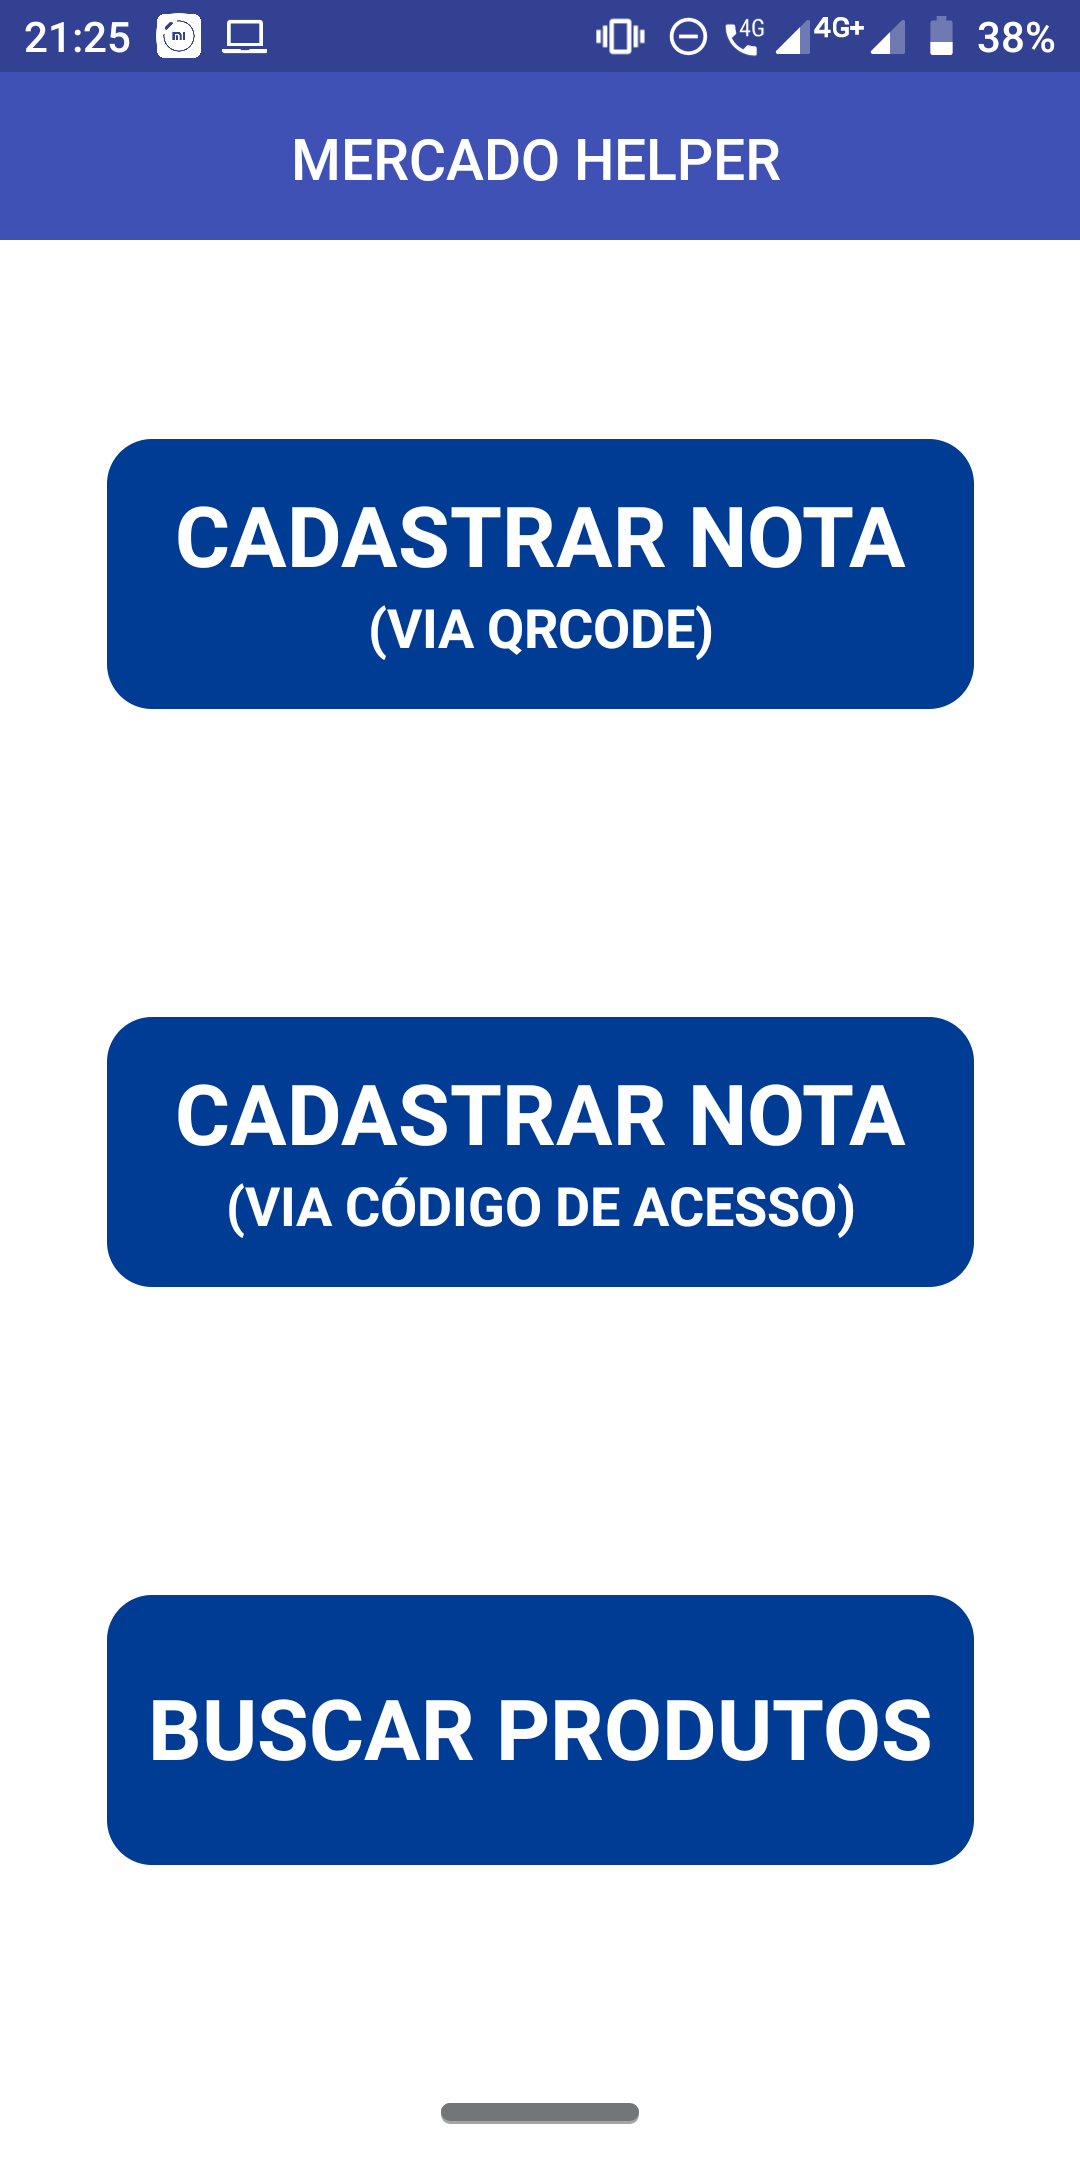
\includegraphics[scale=0.15]{tcc/figures/app/app_home.png}
    \caption{Tela principal}
    \label{appHomeFig}
\end{figure}

\newpage
Após o carregamento desses recursos, o usuário é automaticamente redirecionado para a tela principal do aplicativo, que é demonstrada através da figura \ref{appHomeFig}. A partir dessa tela, é possível efetuar a adição das notas fiscais como a busca por produto através dos atalhos.

No primeiro botão, é possível efetuar a adição da NFC-e através do QRCode presente na mesma. Para tal funcionalidade, é necessário que o dispositivo possua uma câmera e que o usuário conceda permissão para uso da mesma.

No segundo botão, o usuário poderá efetuar a adição através do código de acesso e no último botão, o mesmo poderá consultar a base de dados para obter as informações referentes aos produtos.

\subsection{Adição das notas fiscais}

O usuário poderá efetuar a adição das notas através de duas formas, a primeira que é através do QRCode presente nas versões impressas das mesmas bem como através do código de acesso também disponível na versão física da nota.

Dependendo da forma de adição desejada pelo usuário, o mesmo será redirecionado para outras telas que serão apresentadas logo abaixo.

O meio mais rápido de adicionar é aquele que utiliza o QRCode, pois basta apontar a câmera do smartphone para o código que a leitura do mesmo será feita instantaneamente.

Caso ocorra problemas na leitura desse código, o usuário poderá tentar adicionar através do código de acesso. Esse meio é um pouco mais lento, pois além de inserir esse código de 44 dígitos, será necessário adicionar um código de verificação da solicitação, isto é, o CAPTCHA.

\subsubsection{Através do QRCode}

% FIXME: Ajustar a imagem
% FIXME: Adicionar referencia a imagem
\begin{figure}[h]
    \centering
    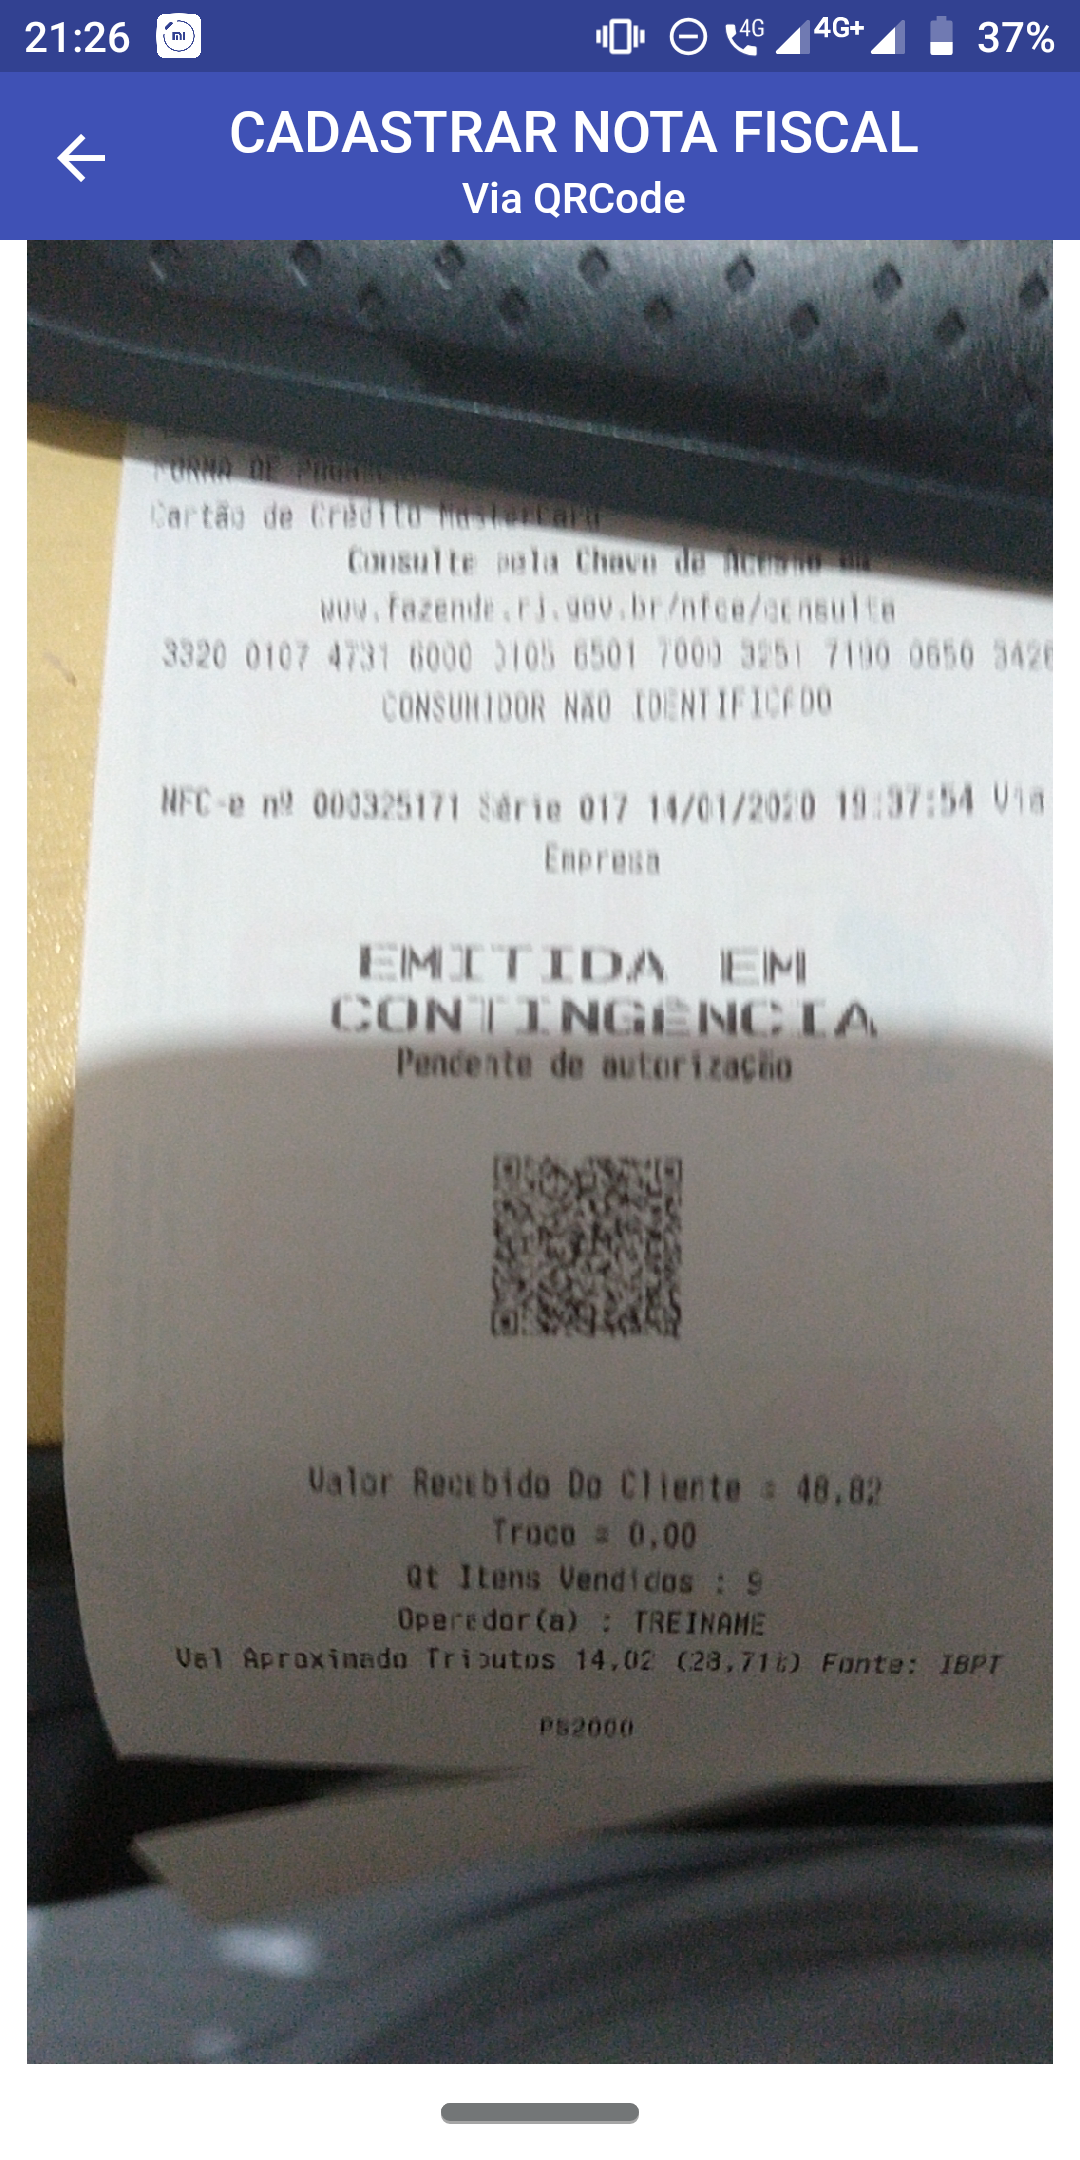
\includegraphics[scale=0.15]{tcc/figures/app/app_codigo_qrcode_solicitacao.png}
    \caption{Exemplo de adição de uma NFC-e real via uso do QRCode}
    \label{appQRCodeSolicitacaoFig}
\end{figure}

Um caso real de adição de uma nota fiscal é representando pela captura da tela do aplicativo no qual é demonstrado pela figura \ref{appQRCodeSolicitacaoFig}. Caso seja feita a detecção do QRCode, o conteúdo contido nesse código será processado e uma solicitação de adição será feita ao servidor.

A latência gerada durante esse período de processamento, faz com seja necessário o uso de uma tela de carregamento. Com isso, é mostrado para o usuário uma barra de progresso que indica que a sua solicitação está sendo processada e o aplicativo continua executando normalmente.

% FIXME: Ajustar a imagem
% FIXME: Adicionar referencia a imagem
\begin{figure}[h]
    \centering
    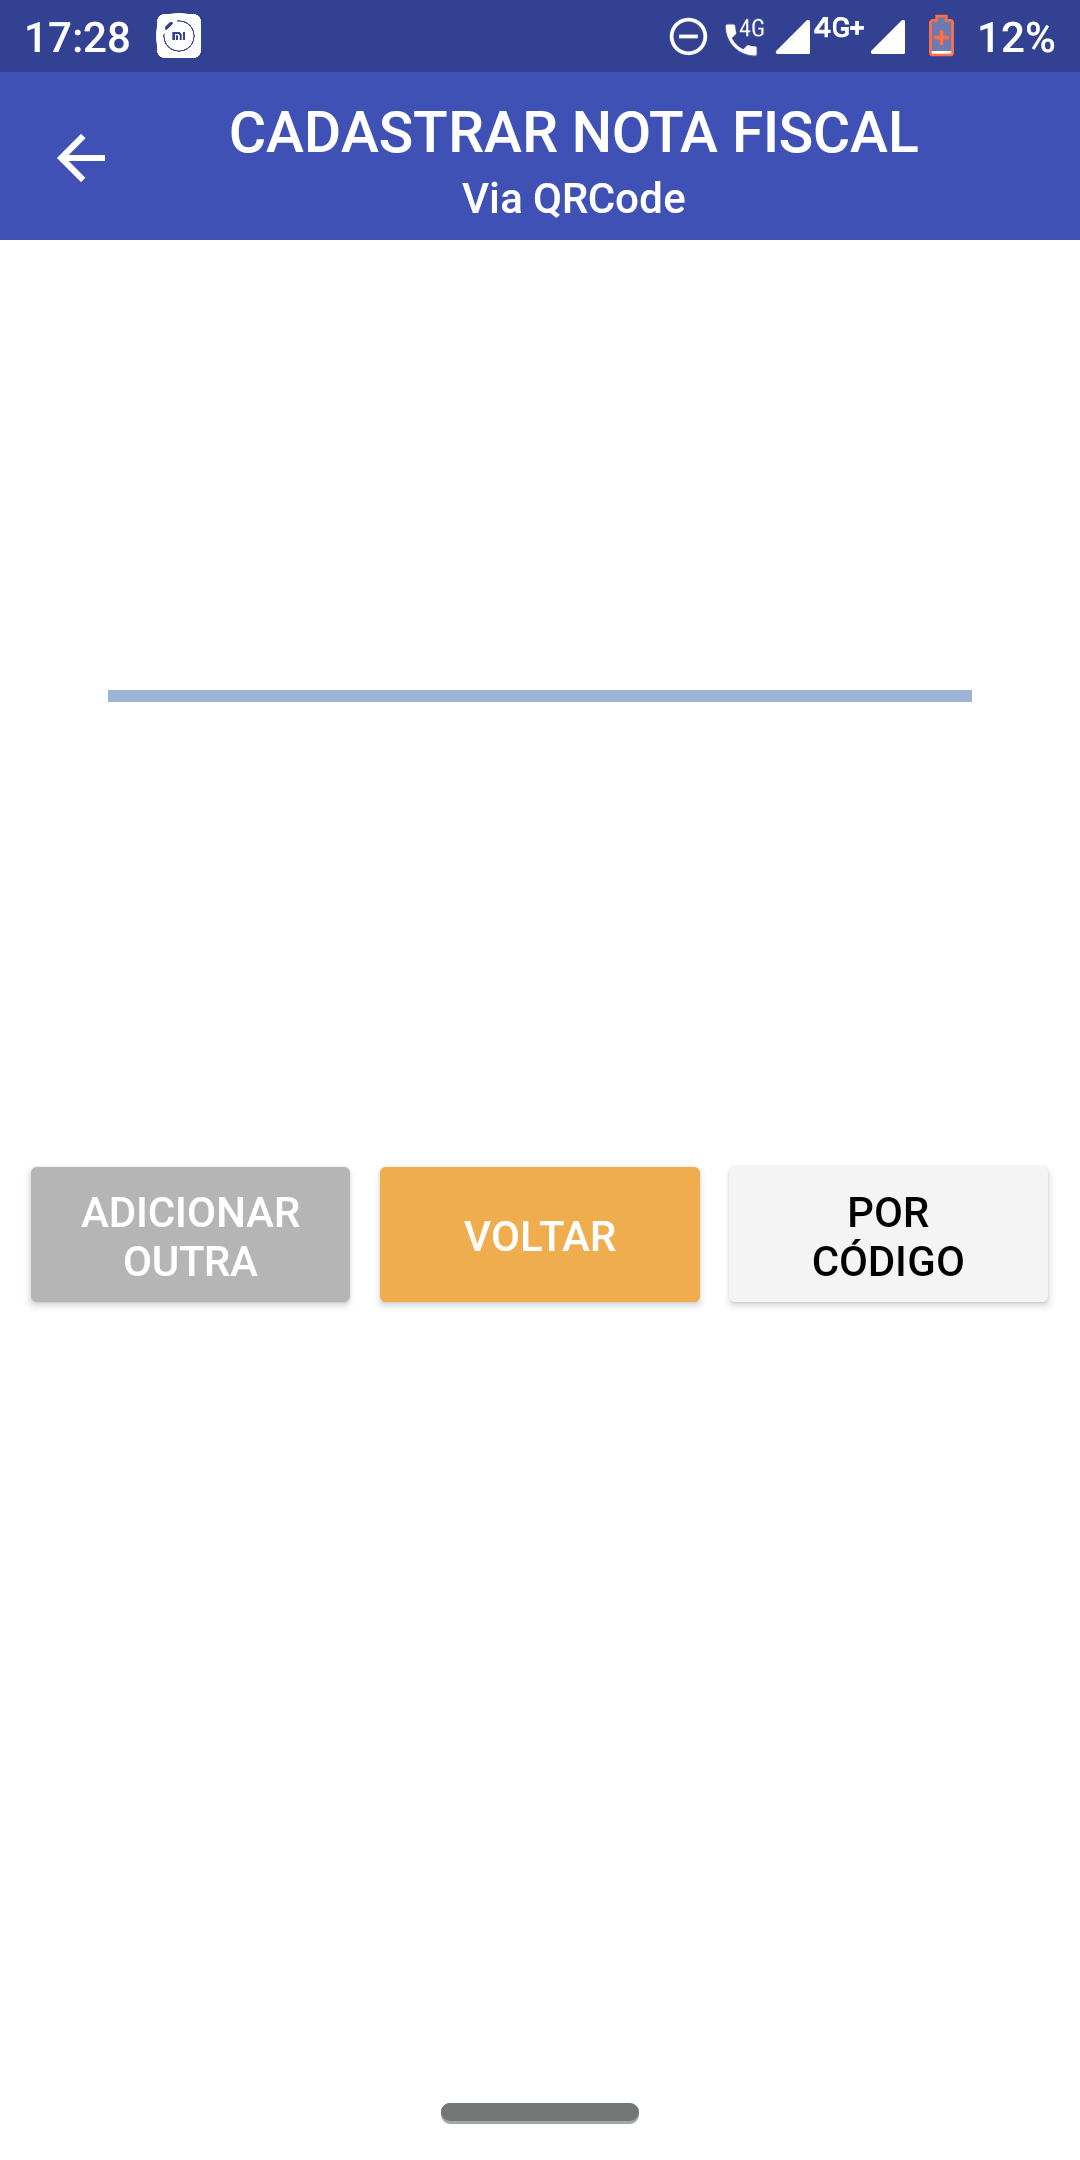
\includegraphics[scale=0.15]{tcc/figures/app/app_codigo_qrcode_loading.png}
    \caption{Tela de cadastro via QRCode após solicitação}
    \label{appQRCodeSolicitacaoFig}
\end{figure}

\newpage
Após o processamento ter terminado, podendo ter sido com sucesso ou não, será enviado para o aplicativo uma resposta contendo o status da solicitação de adição realizada.

Se o código tiver sido lido corretamente e se não houver nenhuma problema durante a solicitação da nota ao site da SEFAZ assim como também no processamento da nota, será mostrado uma mensagem de sucesso conforme pode ser observado na figura abaixo.

% FIXME: Ajustar a imagem
% FIXME: Adicionar referencia a imagem
\begin{figure}[h]
    \centering
    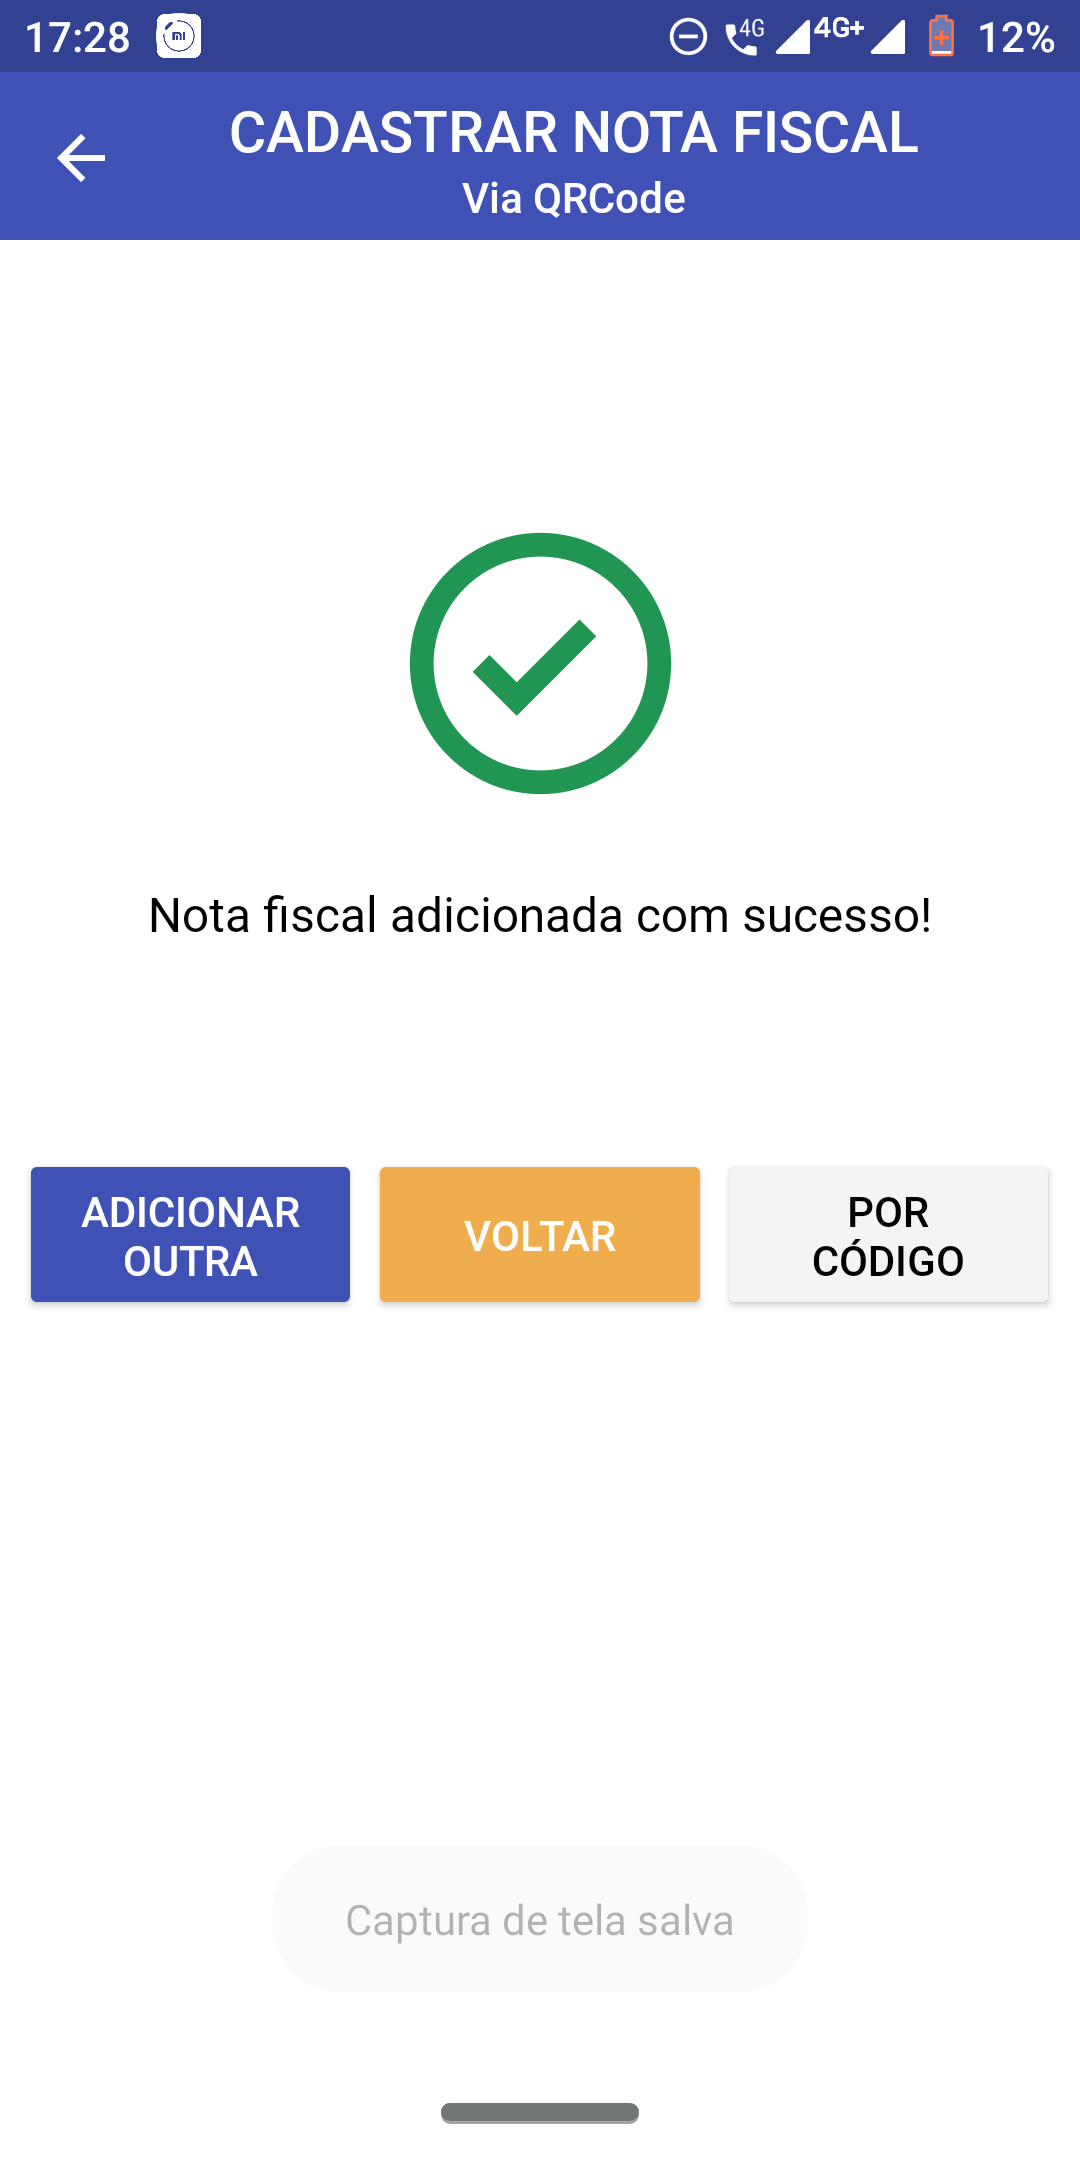
\includegraphics[scale=0.15]{tcc/figures/app/app_codigo_qrcode_sucesso.png}
    \caption{Tela de cadastro efetuado com sucesso}
    \label{appQRCodeSucessoFig}
\end{figure}

\newpage
Todavia, durante o processo de adição, pode ser que a nota ainda não esteja disponível no sistema da SEFAZ, com isso, é feito um tratamento de forma a detectar essa caso, com isso, o usuário será informado que a sua solicitação não foi concluída devido a indisponibilidade em sua versão digital. A figura \ref{appQRCodeNaoDisponivelFig} representa esse caso.

% FIXME: Ajustar a imagem
% FIXME: Trocar por img equivalente do QRCODE
% FIXME: Adicionar referencia a imagem
\begin{figure}[h]
    \centering
    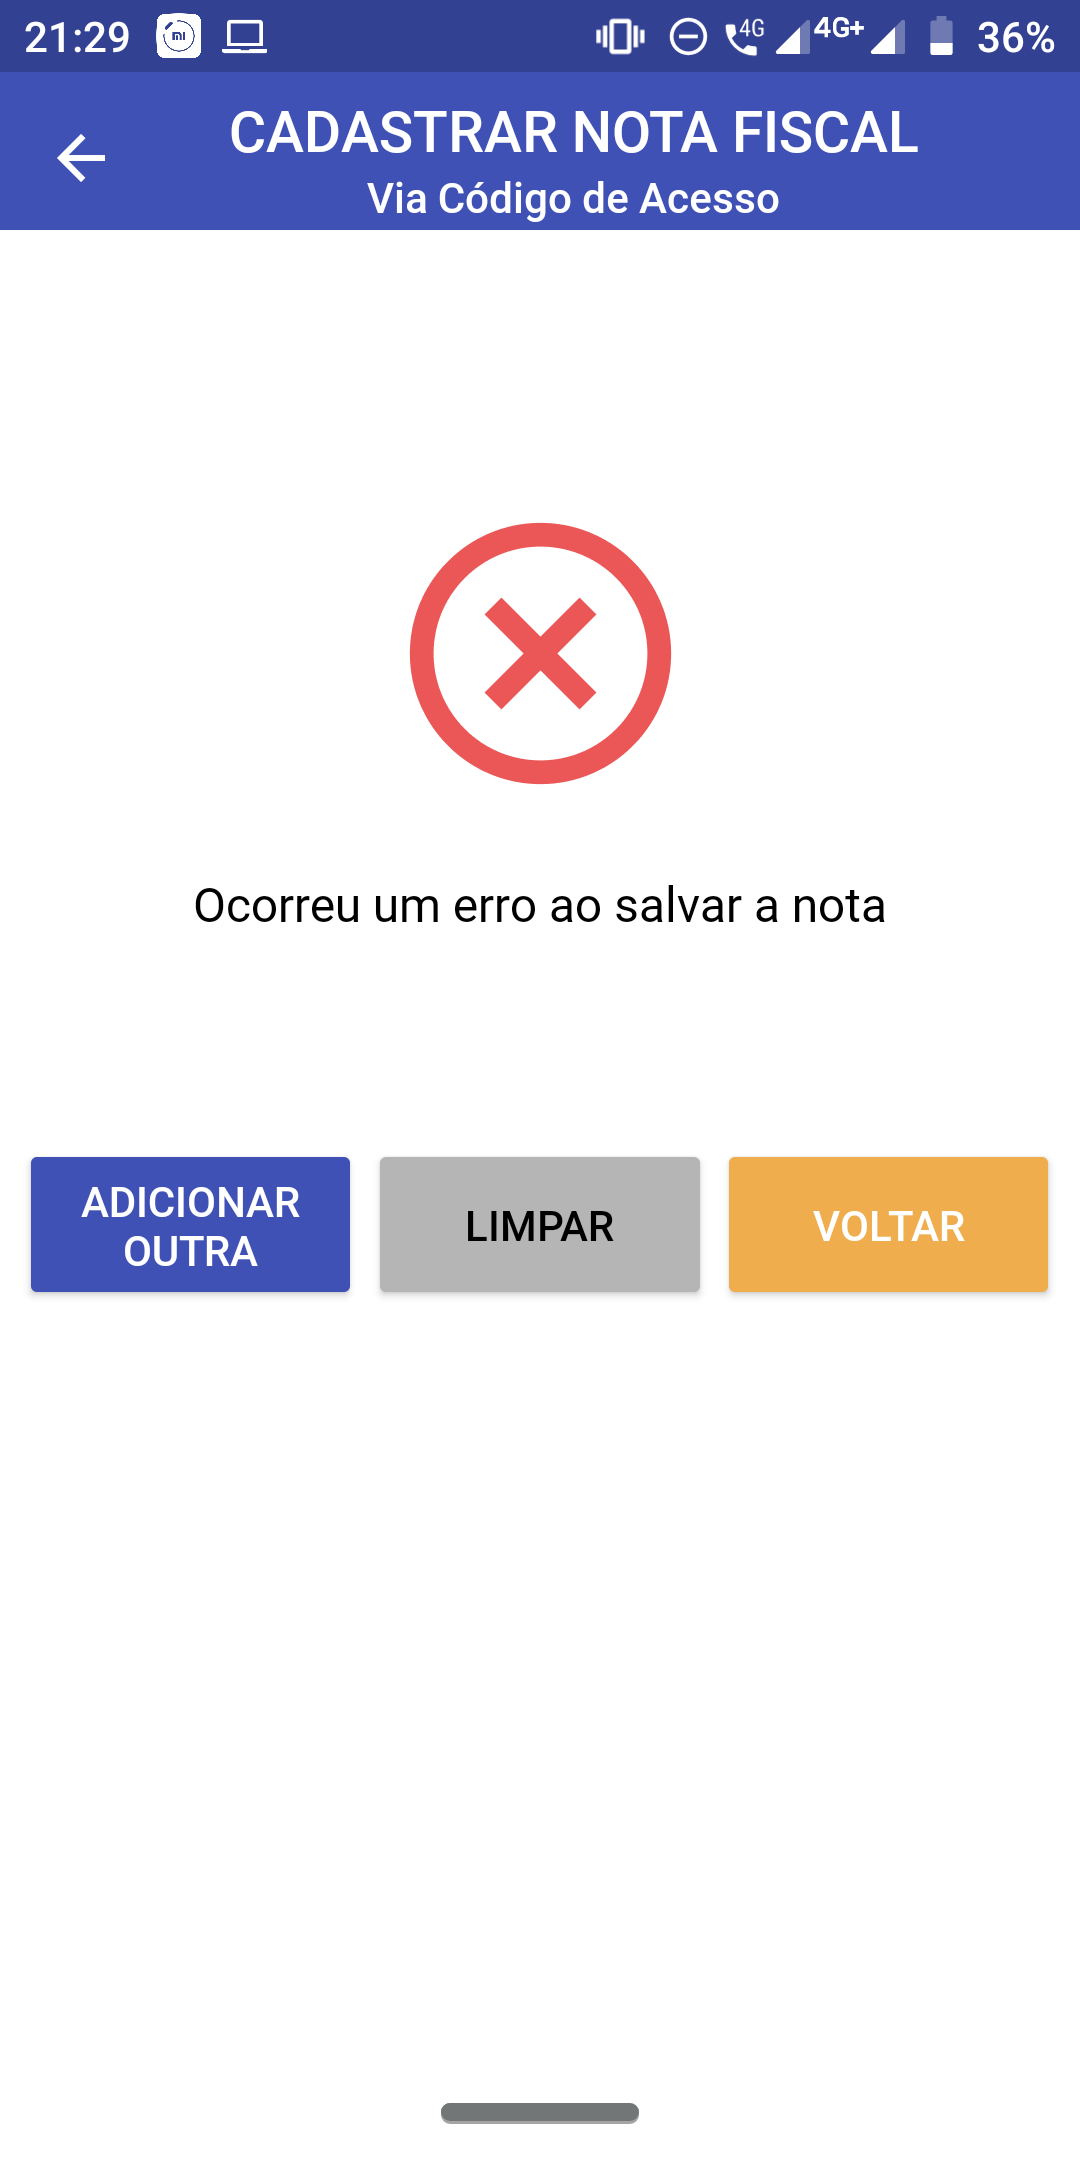
\includegraphics[scale=0.15]{tcc/figures/app/app_codigo_acesso_nao_disponivel.png}
    \caption{Tela de nota não disponível}
    \label{appQRCodeNaoDisponivelFig}
\end{figure}

\newpage
Uma outra situação que poderá ocorrer, é caso o usuário tente adicionar uma nota que já foi adicionada previamente. A solicitação ao sistema da SEFAZ será feita normalmente até a obtenção do código de acesso da NFC-e, que é um código único. Após a aquisição desse código, é feita uma pesquisa no banco de dados de forma a verificar a existência dessa nota nos registros. Caso a nota seja encontrada, será enviado ao aplicativo um código de erro indicando a existência dessa nota, com isso o usuário poderá visualizar a tela da figura \ref{appQRCodeJaCadastradaFig}. Para o caso contrário, isto é, que a nota não é encontrada, seguirá com o fluxo normal.

% FIXME: Ajustar a imagem
% FIXME: Adicionar referencia a imagem
\begin{figure}[h]
    \centering
    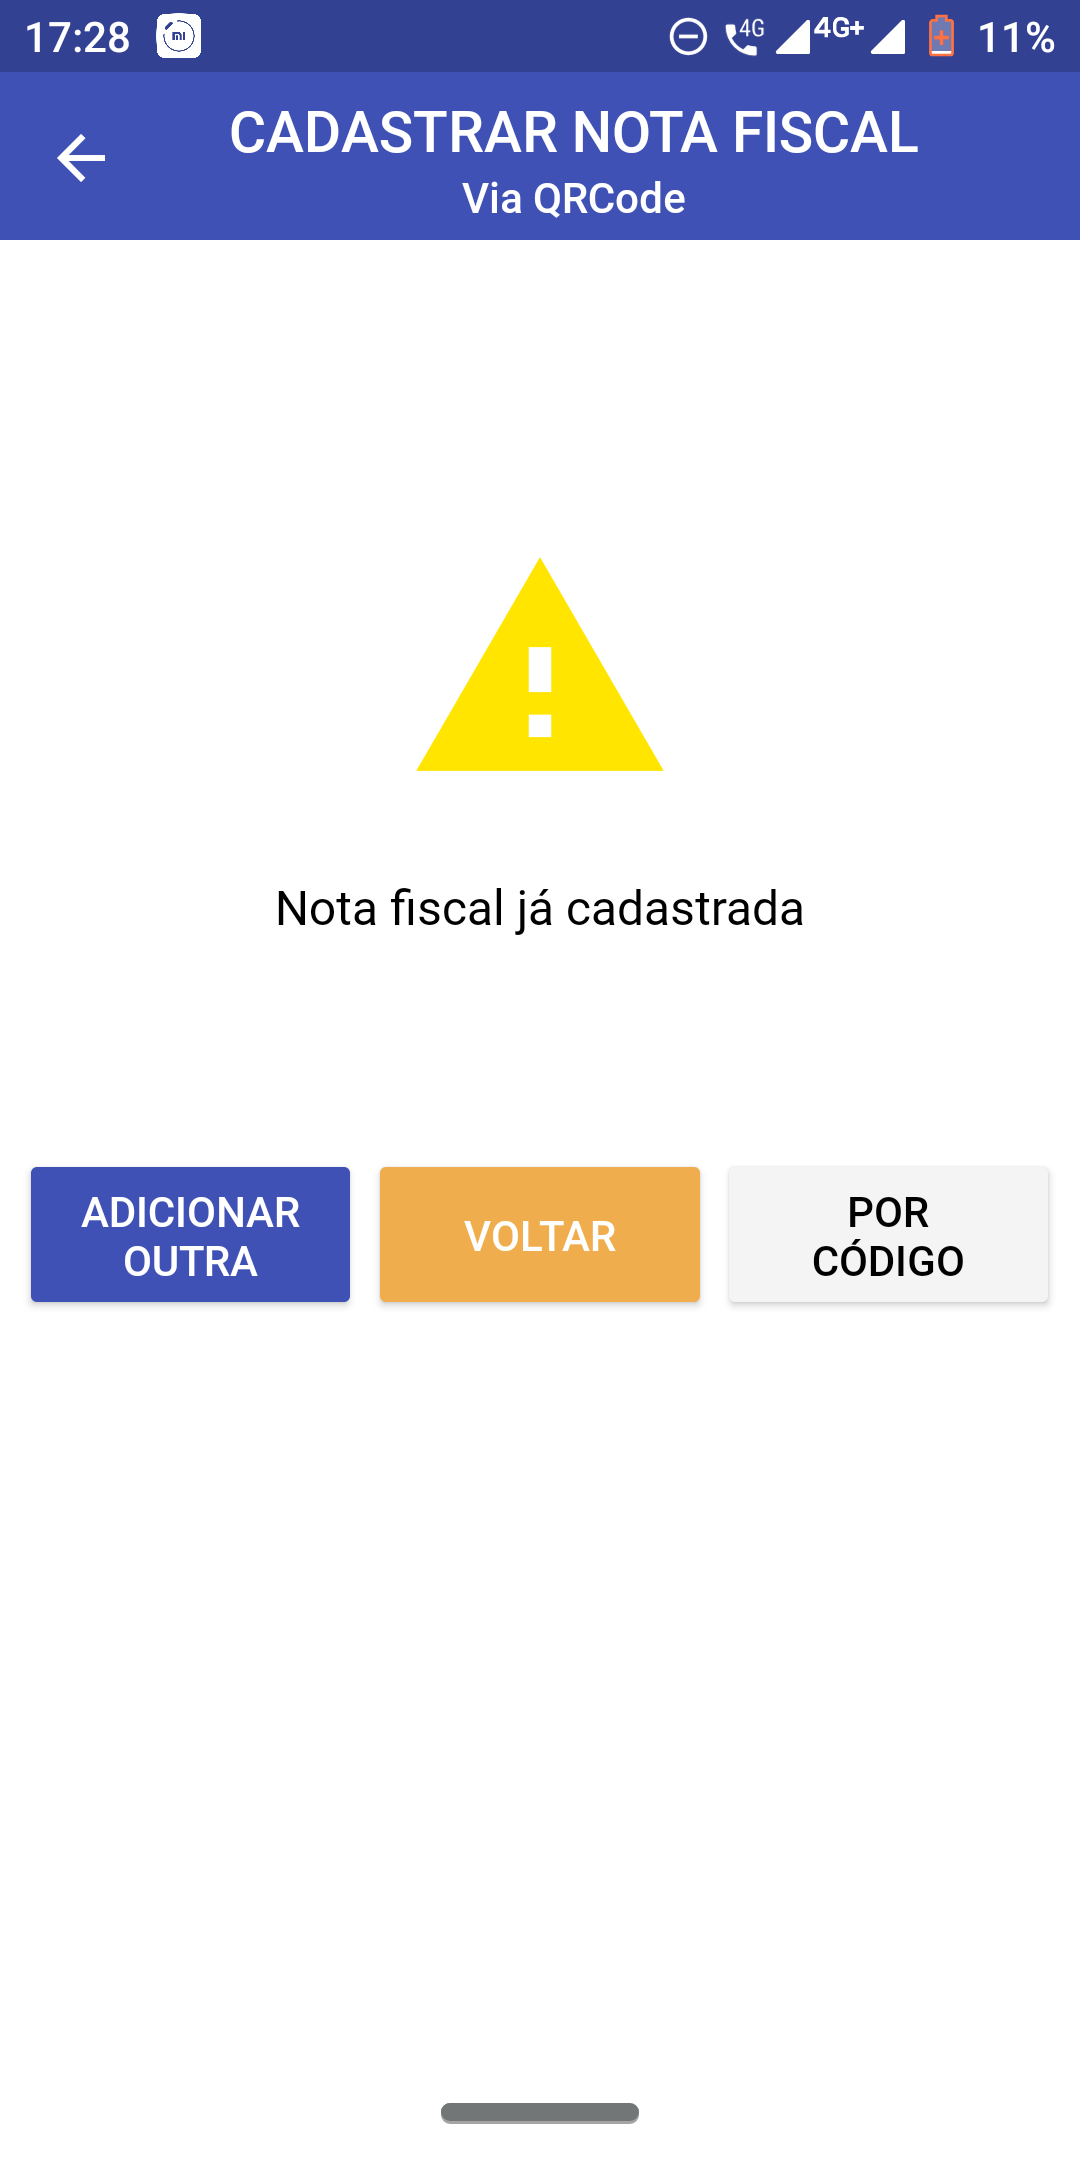
\includegraphics[scale=0.15]{tcc/figures/app/app_codigo_qrcode_ja_cadastrada.png}
    \caption{Tela de nota já cadastrada previamente}
    \label{appQRCodeJaCadastradaFig}
\end{figure}

\newpage
Durante a solicitação, está suscetível a ocorrência de erros, que pode se dar devido a problemas com a rede, problemas no sistema da SEFAZ e entre outras inúmeras situações. Diante desses erros inesperados, o usuário também é informado através de uma mensagem de erro genérica.

% FIXME: Ajustar a imagem
% FIXME: Adicionar referencia a imagem
\begin{figure}[h]
    \centering
    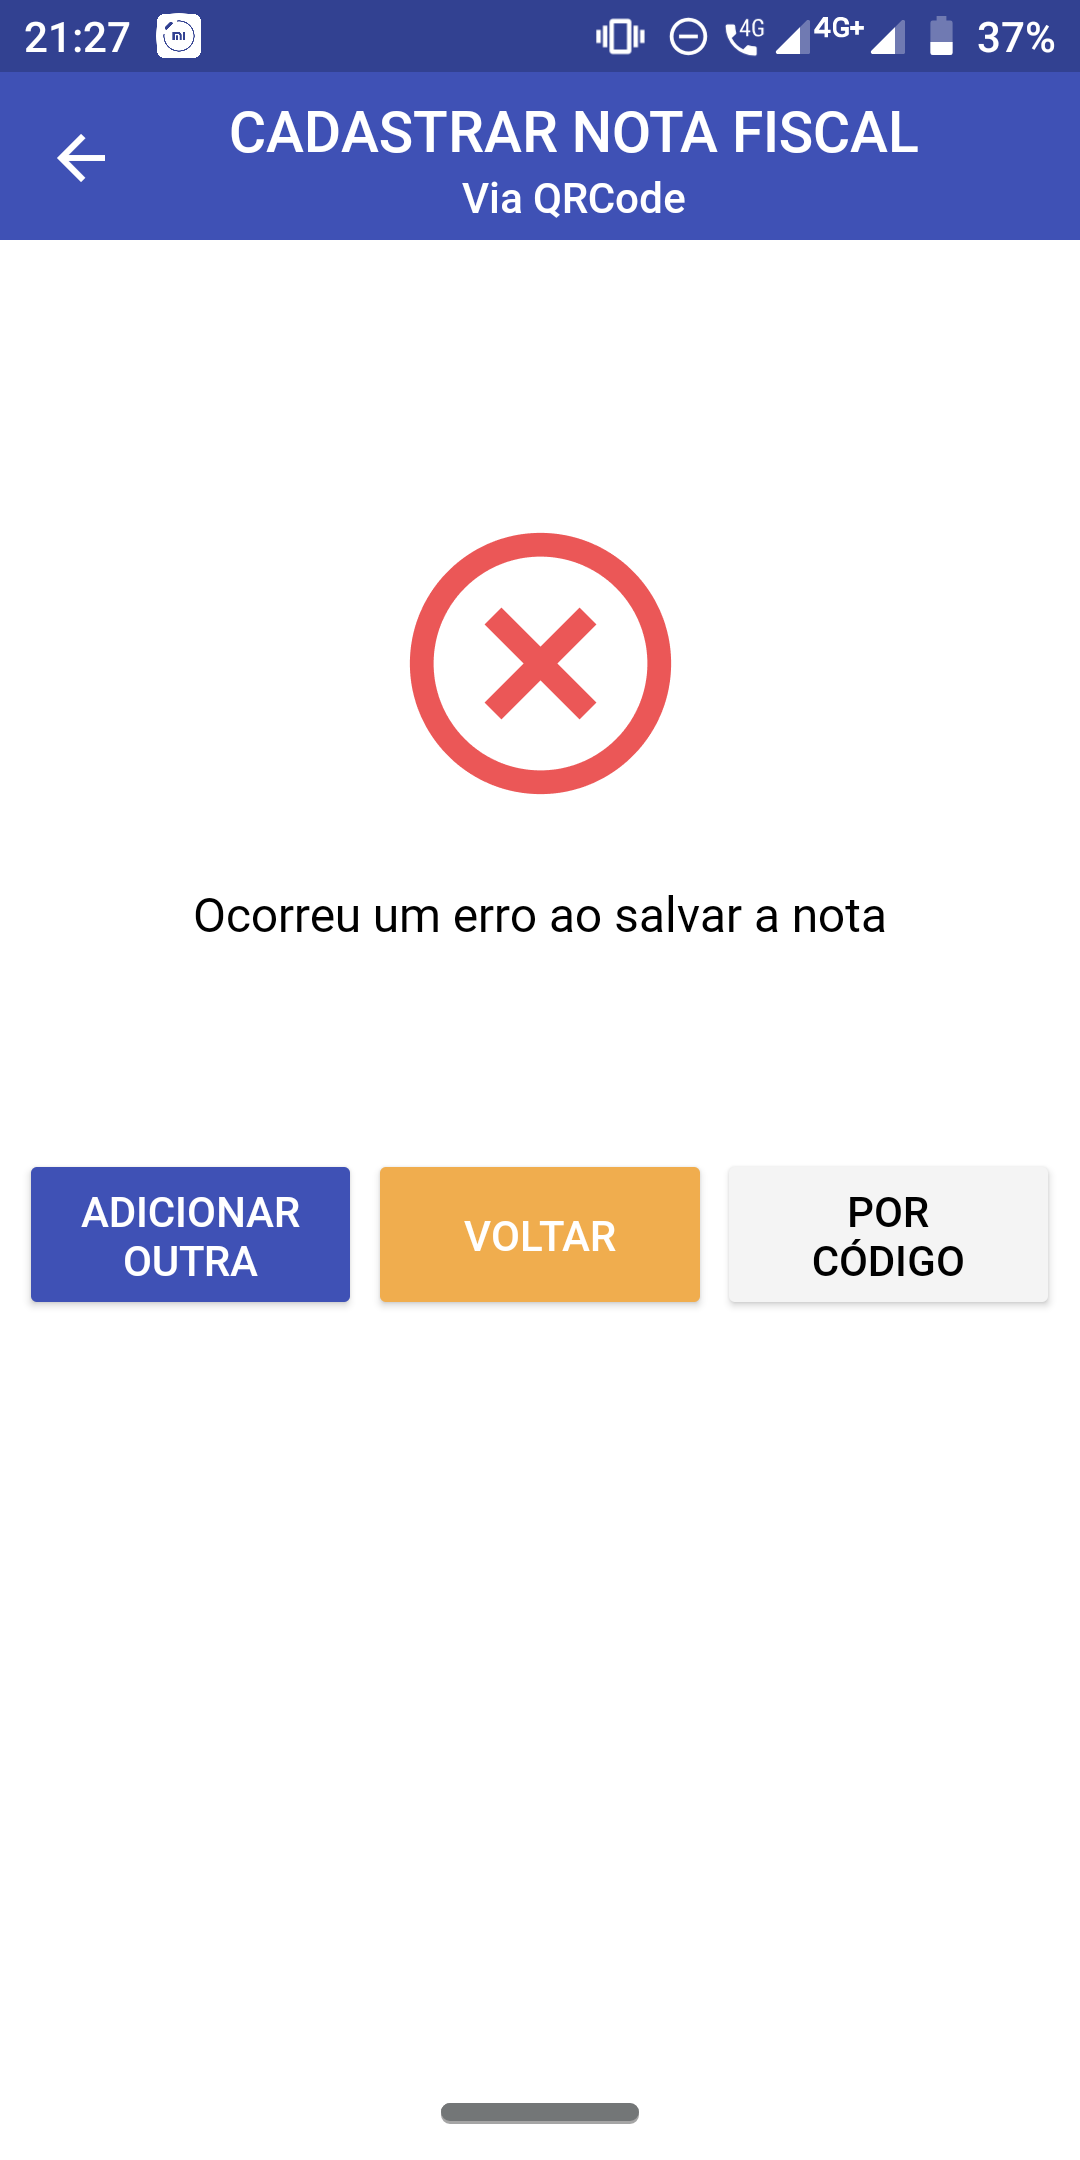
\includegraphics[scale=0.15]{tcc/figures/app/app_codigo_qrcode_erro.png}
    \caption{Tela apresentada após erro durante solicitação}
    \label{appQRCodeErroFig}
\end{figure}

\newpage
Em suma, vale destacar que, independente do caso, é apresentado ao usuário três opções, através de botões, após o término do processamento da solicitação. A primeira opção, representada pelo botão azul, permite ao usuário adicionar uma outra nota fiscal através do uso do QRCode ou até mesmo tentar adicionar a mesma nota novamente caso tenha ocorrido erros. A opção do meio, isto é, pelo botão amarelo, permite que o usuário retorne para a tela inicial. Por fim, o último botão, representa um atalho para adição através do uso do código de acesso.

\subsubsection{Através de código de acesso}

Se durante o processo de impressão da NFC-e ocorrer problemas e o QRCode não ficar nítido ou apresentar falhas, o aplicativo estará propenso a não conseguir efetuar a leitura correta da informação presente nesse código. Para contornar esse problema, é oferecida uma outra forma de adição de notas através de uma outra informação também presente na mesma, isto é, através do código de acesso.

\newpage
% FIXME: Ajustar a imagem
% FIXME: Adicionar referencia a imagem
\begin{figure}[h]
    \centering
    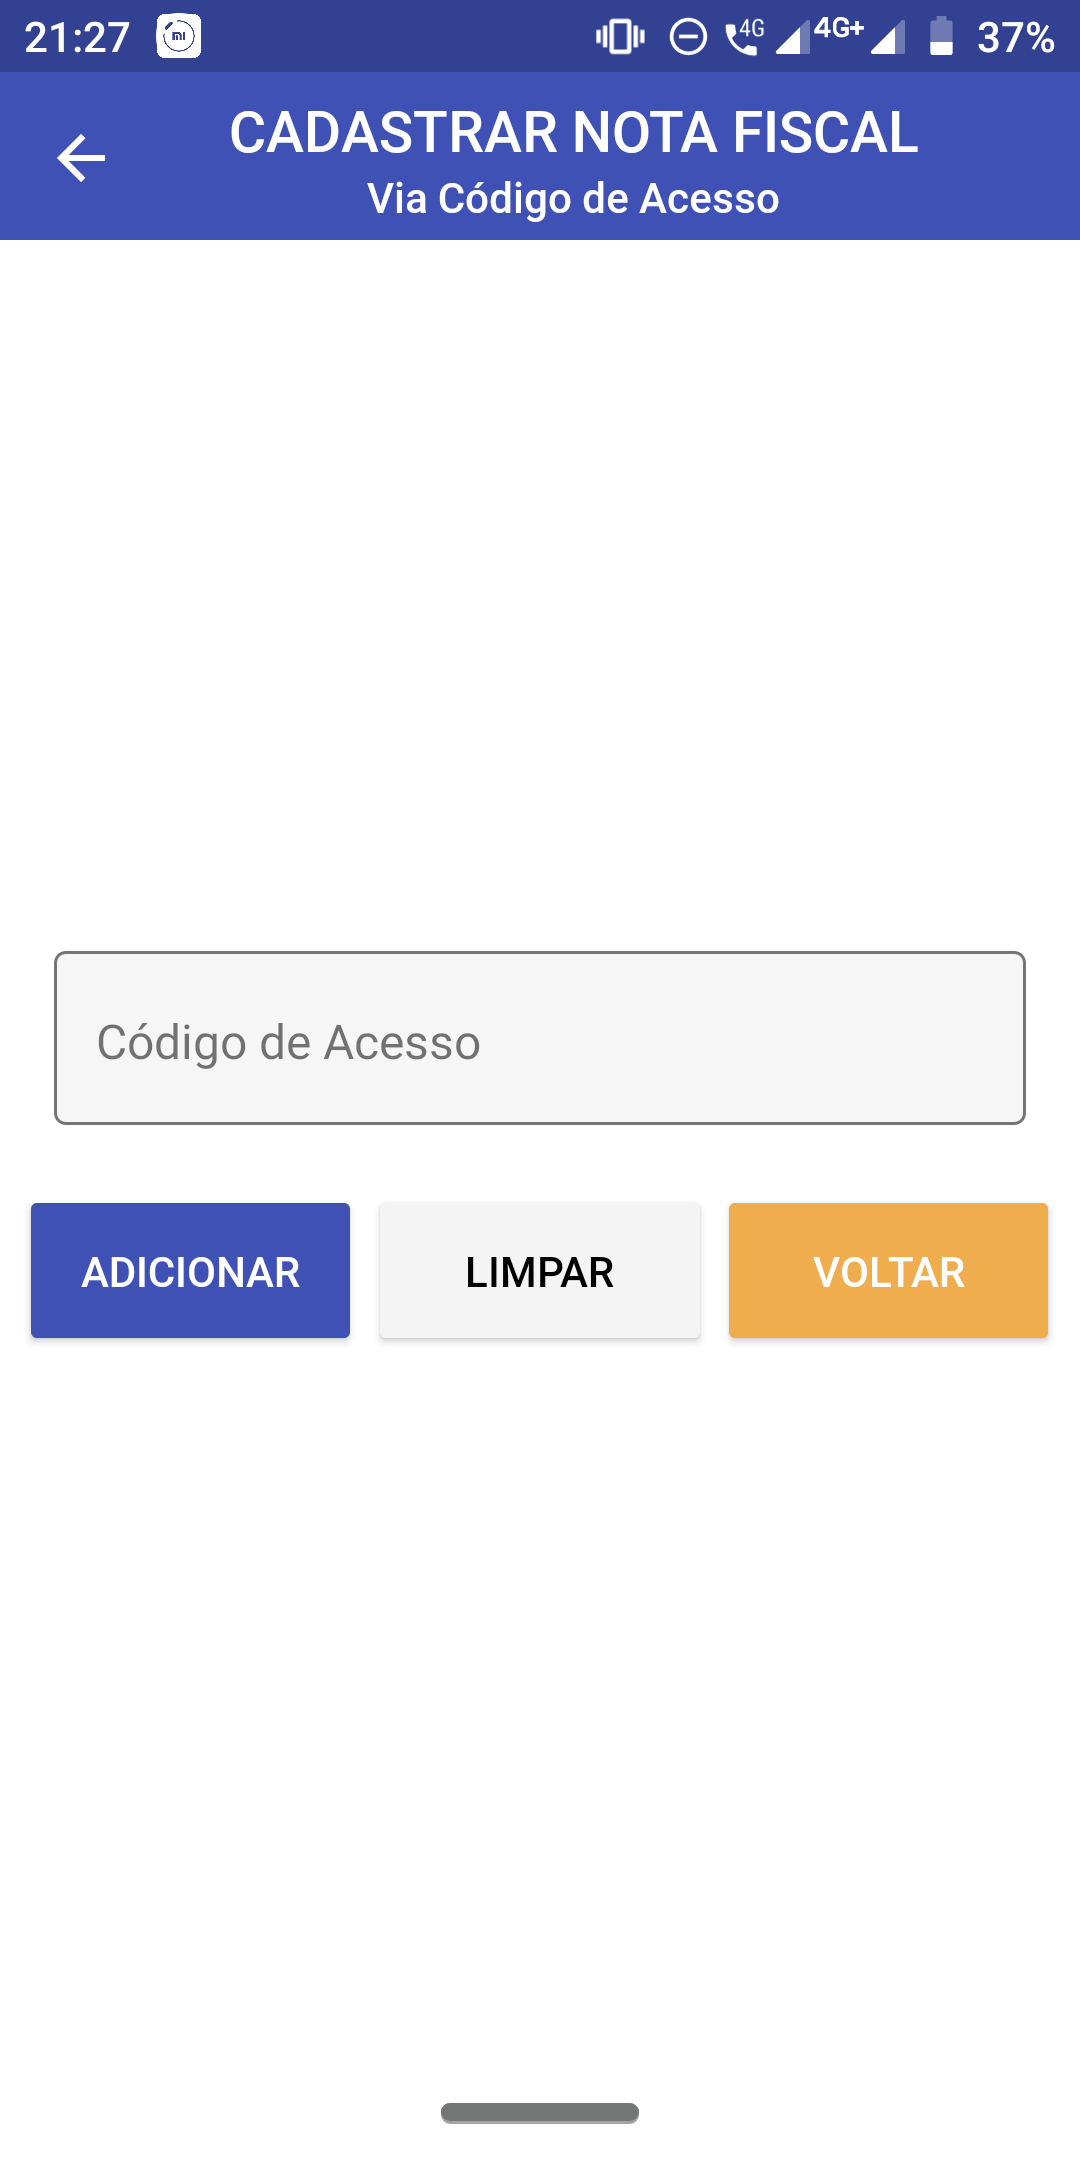
\includegraphics[scale=0.15]{tcc/figures/app/app_codigo_acesso.png}
    \caption{Tela inicial do cadastro via código de acesso}
    \label{appCodigoAcessoInicialFig}
\end{figure}

A figura \ref{appCodigoAcessoInicialFig} representa a tela inicial de cadastro efetuado através do uso do código de acesso. O primeiro campo é para a inserção do código que é necessário para solicitação. Abaixo desse campo, encontram-se os botões para a interação do usuário. O primeiro botão, em azul, é para a inicialização do processo de adição. Caso o usuário não insira a quantidade necessária de dígitos, o sistema irá notificar o usuário sobre esse problema. O botão do meio, em branco, permite a limpeza total do texto inserido. Por último, o botão mais à direita serve como atalho para o usuário retornar à tela inicial.

\newpage
% FIXME: Ajustar a imagem
% FIXME: Adicionar referencia a imagem
\begin{figure}[h]
    \centering
    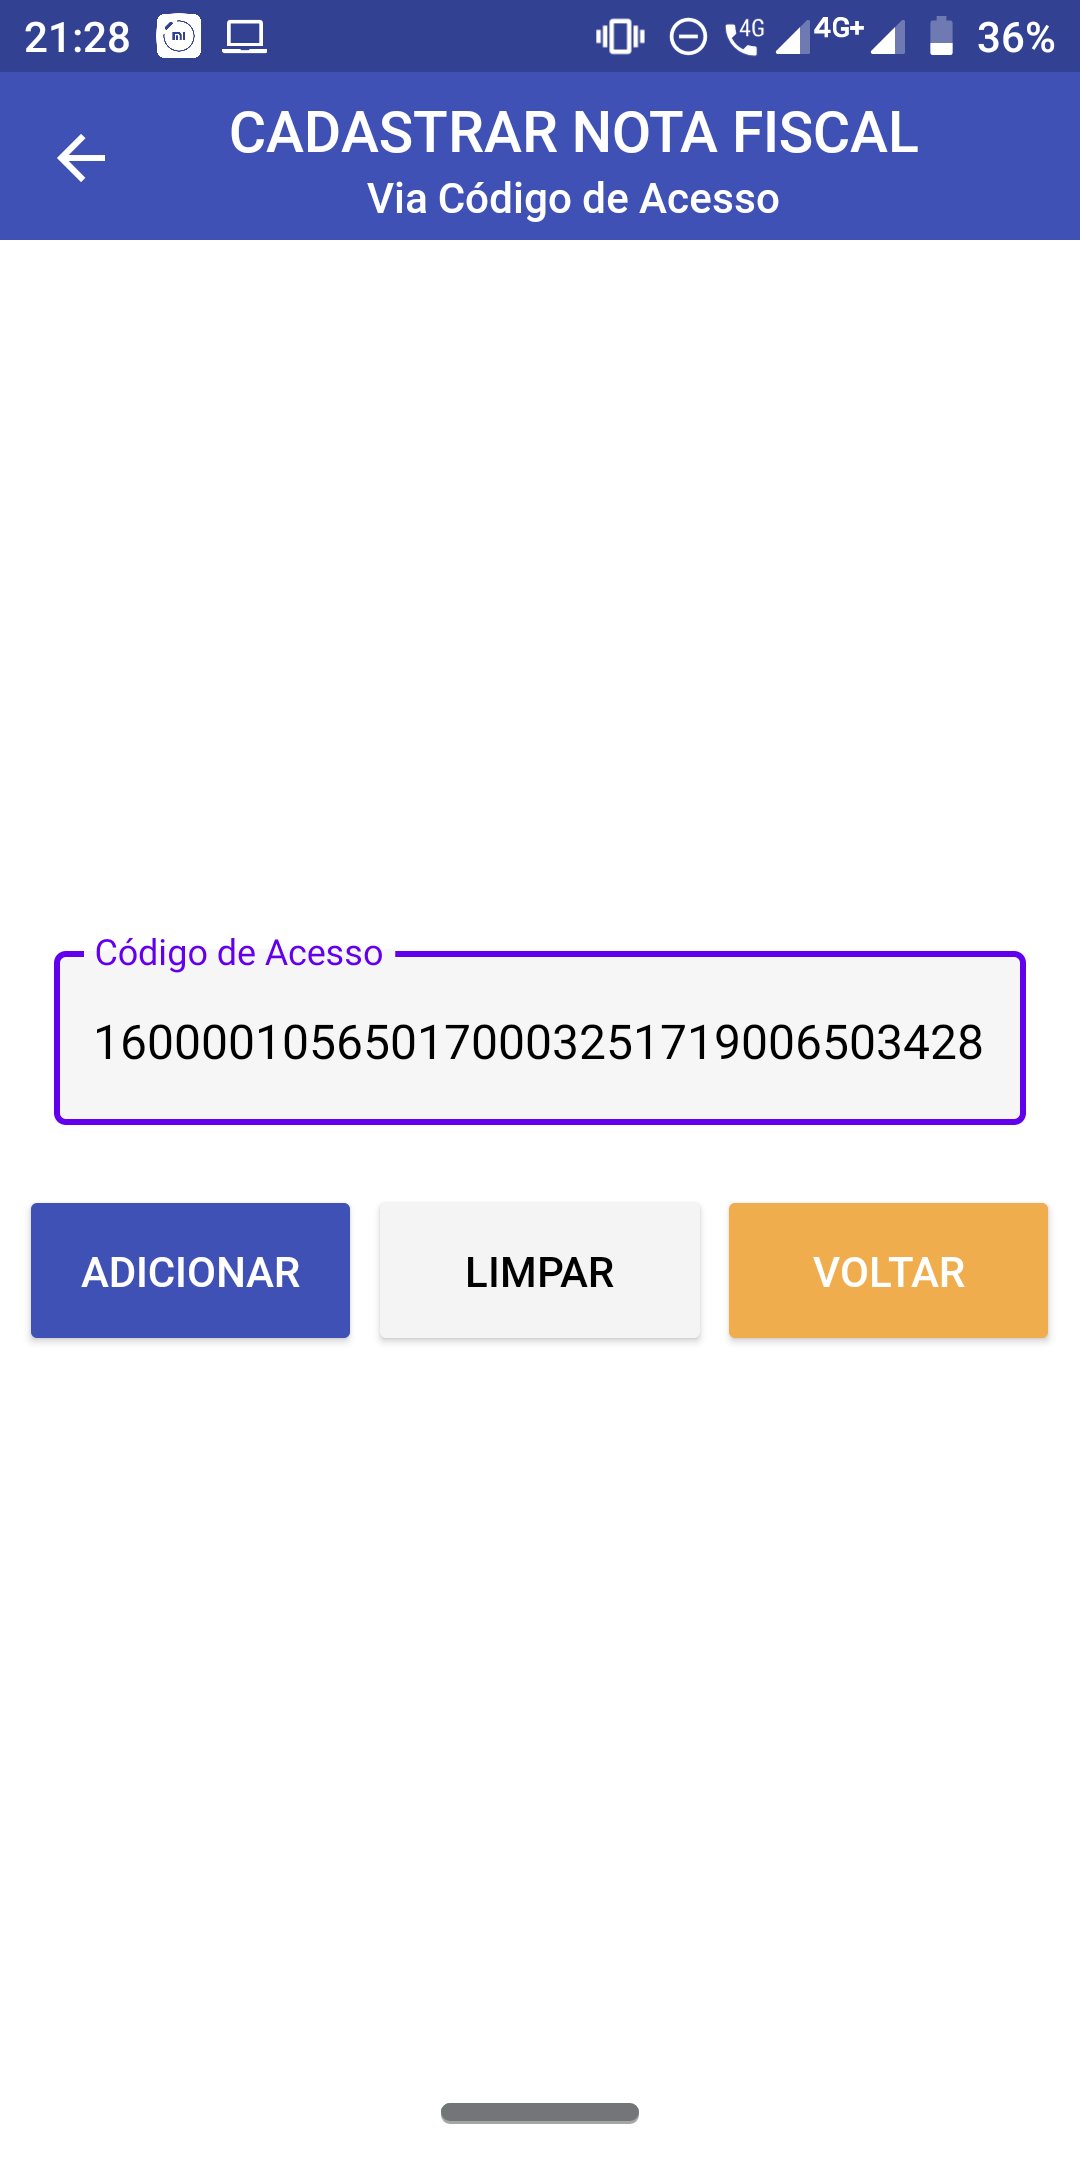
\includegraphics[scale=0.15]{tcc/figures/app/app_codigo_acesso_com_codigo.png}
    \caption{Tela de cadastro via código de acesso com código inserido}
    \label{appCodigoAcessoComCodigoFig}
\end{figure}

% FIXME: Ajustar a imagem
% FIXME: Adicionar referencia a imagem
\begin{figure}[h]
    \centering
    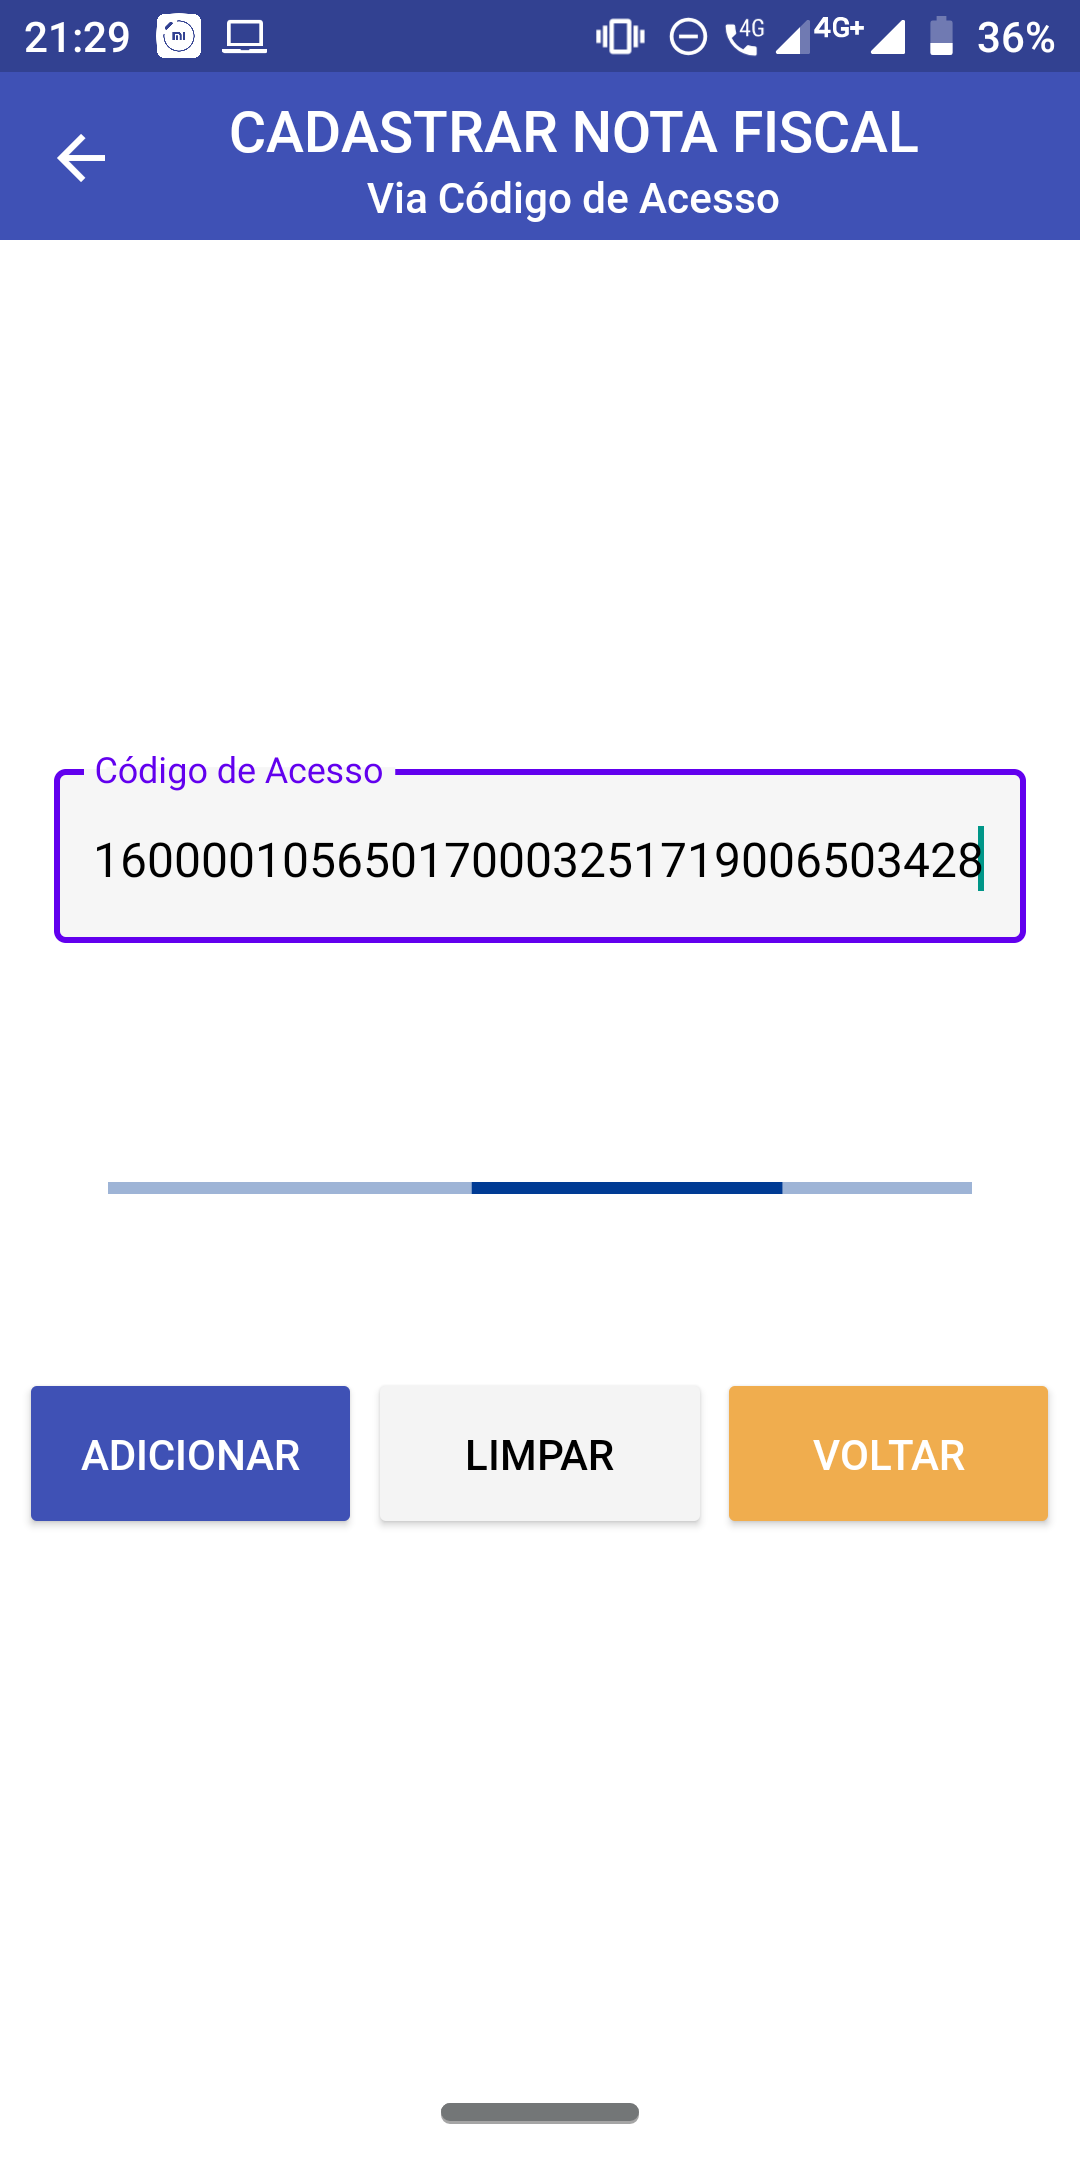
\includegraphics[scale=0.15]{tcc/figures/app/app_codigo_acesso_loading.png}
    \caption{Tela de cadastro via código de acesso com carregamento}
    \label{appCodigoAcessoCarregamentoCaptchaFig}
\end{figure}

\newpage
Após a inserção do código de acesso e o usuário ter pressionado o botão de adicionar, será mostrado o CAPTCHA para validação da requisição. Esse código é necessário para comprovação que a solicitação é proveniente de interação humana e não foi feita por sistemas automáticos. Essa validação pertence ao sistema da SEFAZ e o aplicativo simplesmente replica a mesma imagem utilizada por esse sistema para que a solicitação efetuada no site possa ser simulada. Como essa imagem precisa ser transferida para o aplicativo, uma barra de progresso é exibida até que a imagem seja baixada em sua totalidade conforme é explicitado pela Figura \ref{appCodigoAcessoCarregamentoCaptchaFig}. Além da imagem representativa desse código de validação, um campo destinado a inserção do texto referente a essa mesma imagem são acrescentados à tela anterior. A figura \ref{appCodigoAcessoCaptchaFig} exemplifica esse fluxo descrito.

Vale destacar, que os mesmos botões disponíveis na tela anterior (Figura \ref{appCodigoAcessoComCodigoFig}) ainda estão presentes, todavia, o botão de adicionar deverá ser utilizado após a inserção do texto referente ao CAPTCHA, já o botão limpar serve para limpeza do campo destinado a inserção desse mesmo texto.

\newpage
% FIXME: Ajustar a imagem
% FIXME: Adicionar referencia a imagem
\begin{figure}[h]
    \centering
    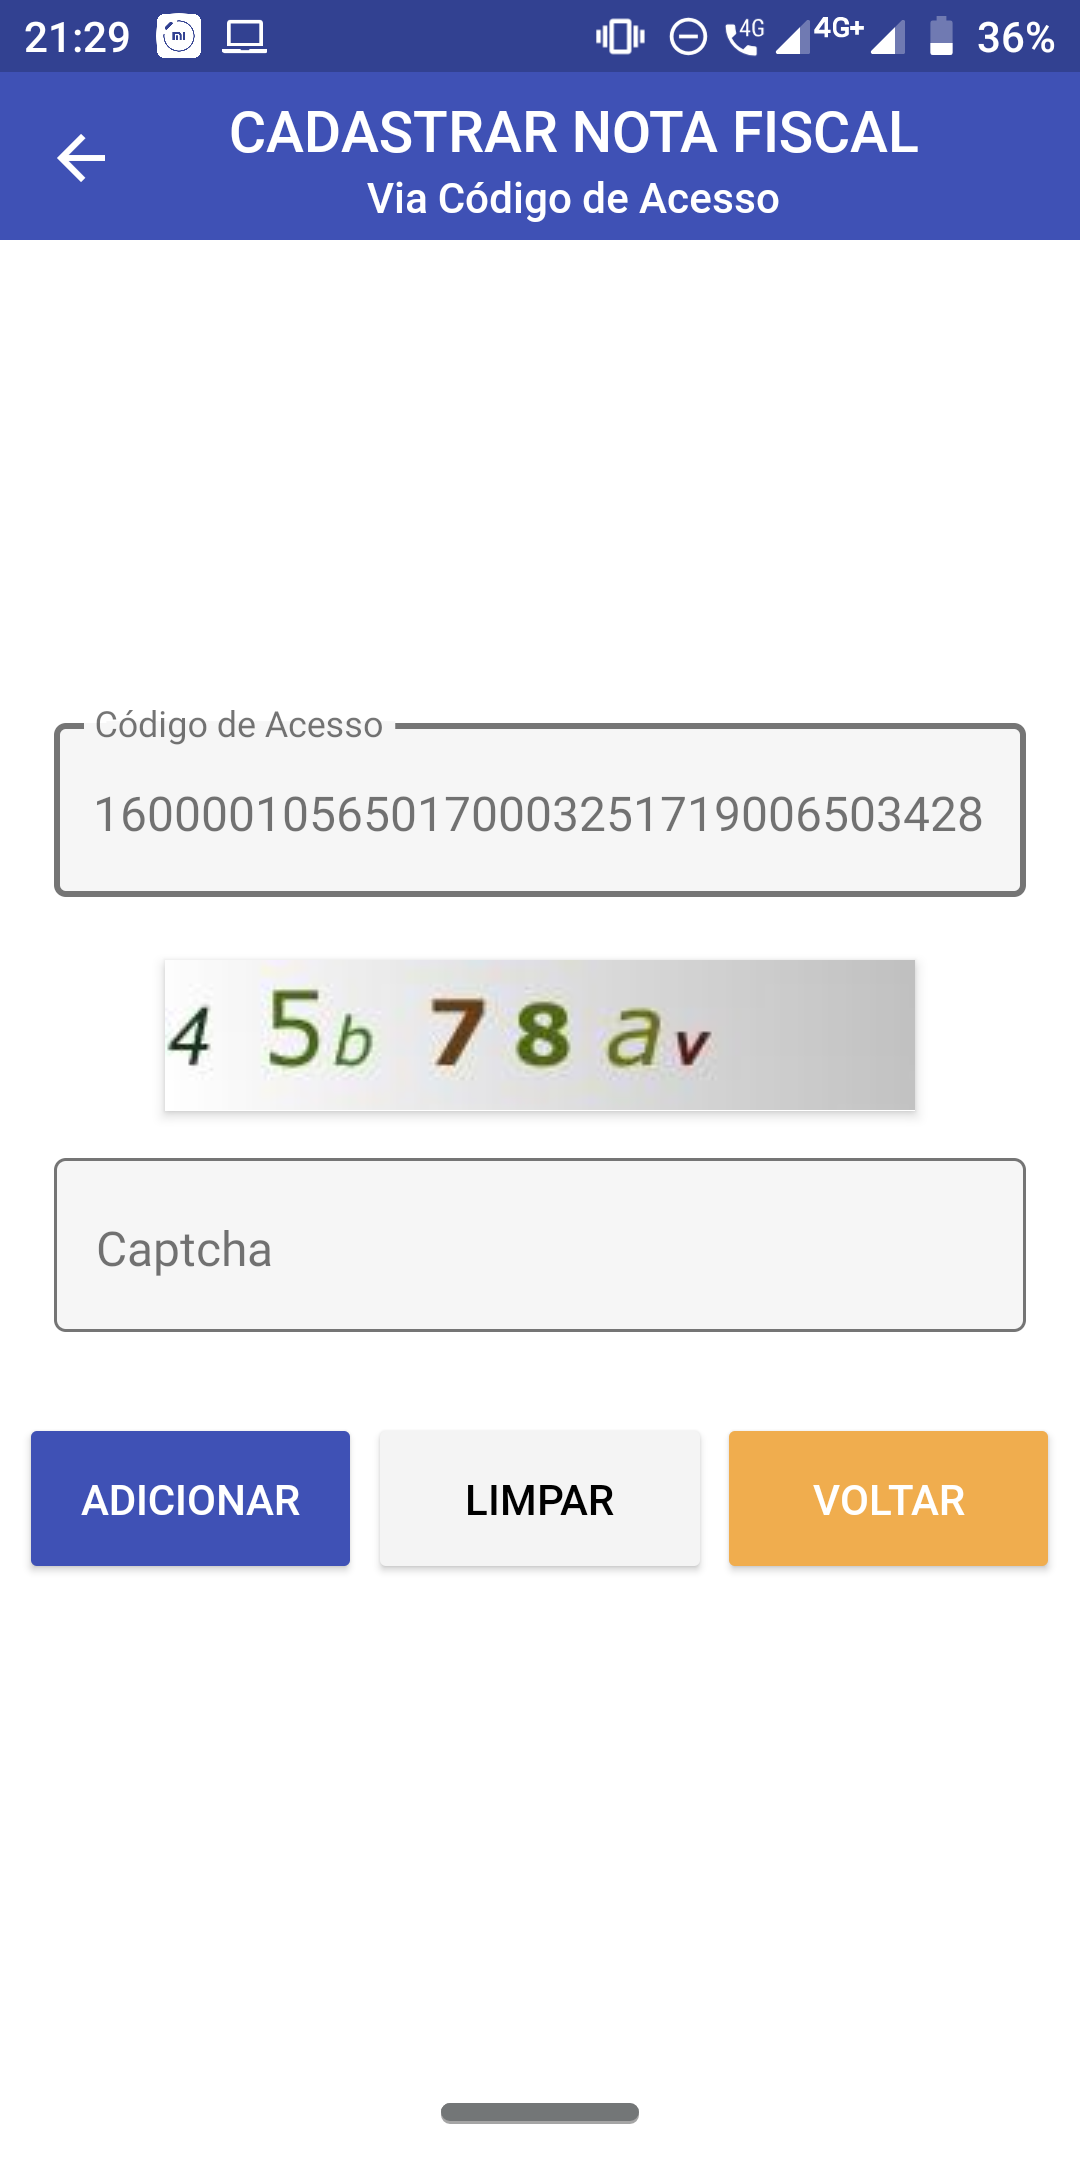
\includegraphics[scale=0.15]{tcc/figures/app/app_codigo_acesso_captcha.png}
    \caption{Tela de cadastro solicitando CAPTCHA para validação da requisição}
    \label{appCodigoAcessoCaptchaFig}
\end{figure}

Assim como ocorre com o cadastro via QRCode, alguns segundos serão gastos até o término do processamento dos dados, com isso, uma tela com uma barra de progresso também é exibida até o resultado da solicitação ser retornado ao aplicativo.

\newpage
% FIXME: Ajustar a imagem
% FIXME: Adicionar referencia a imagem
\begin{figure}[h]
    \centering
    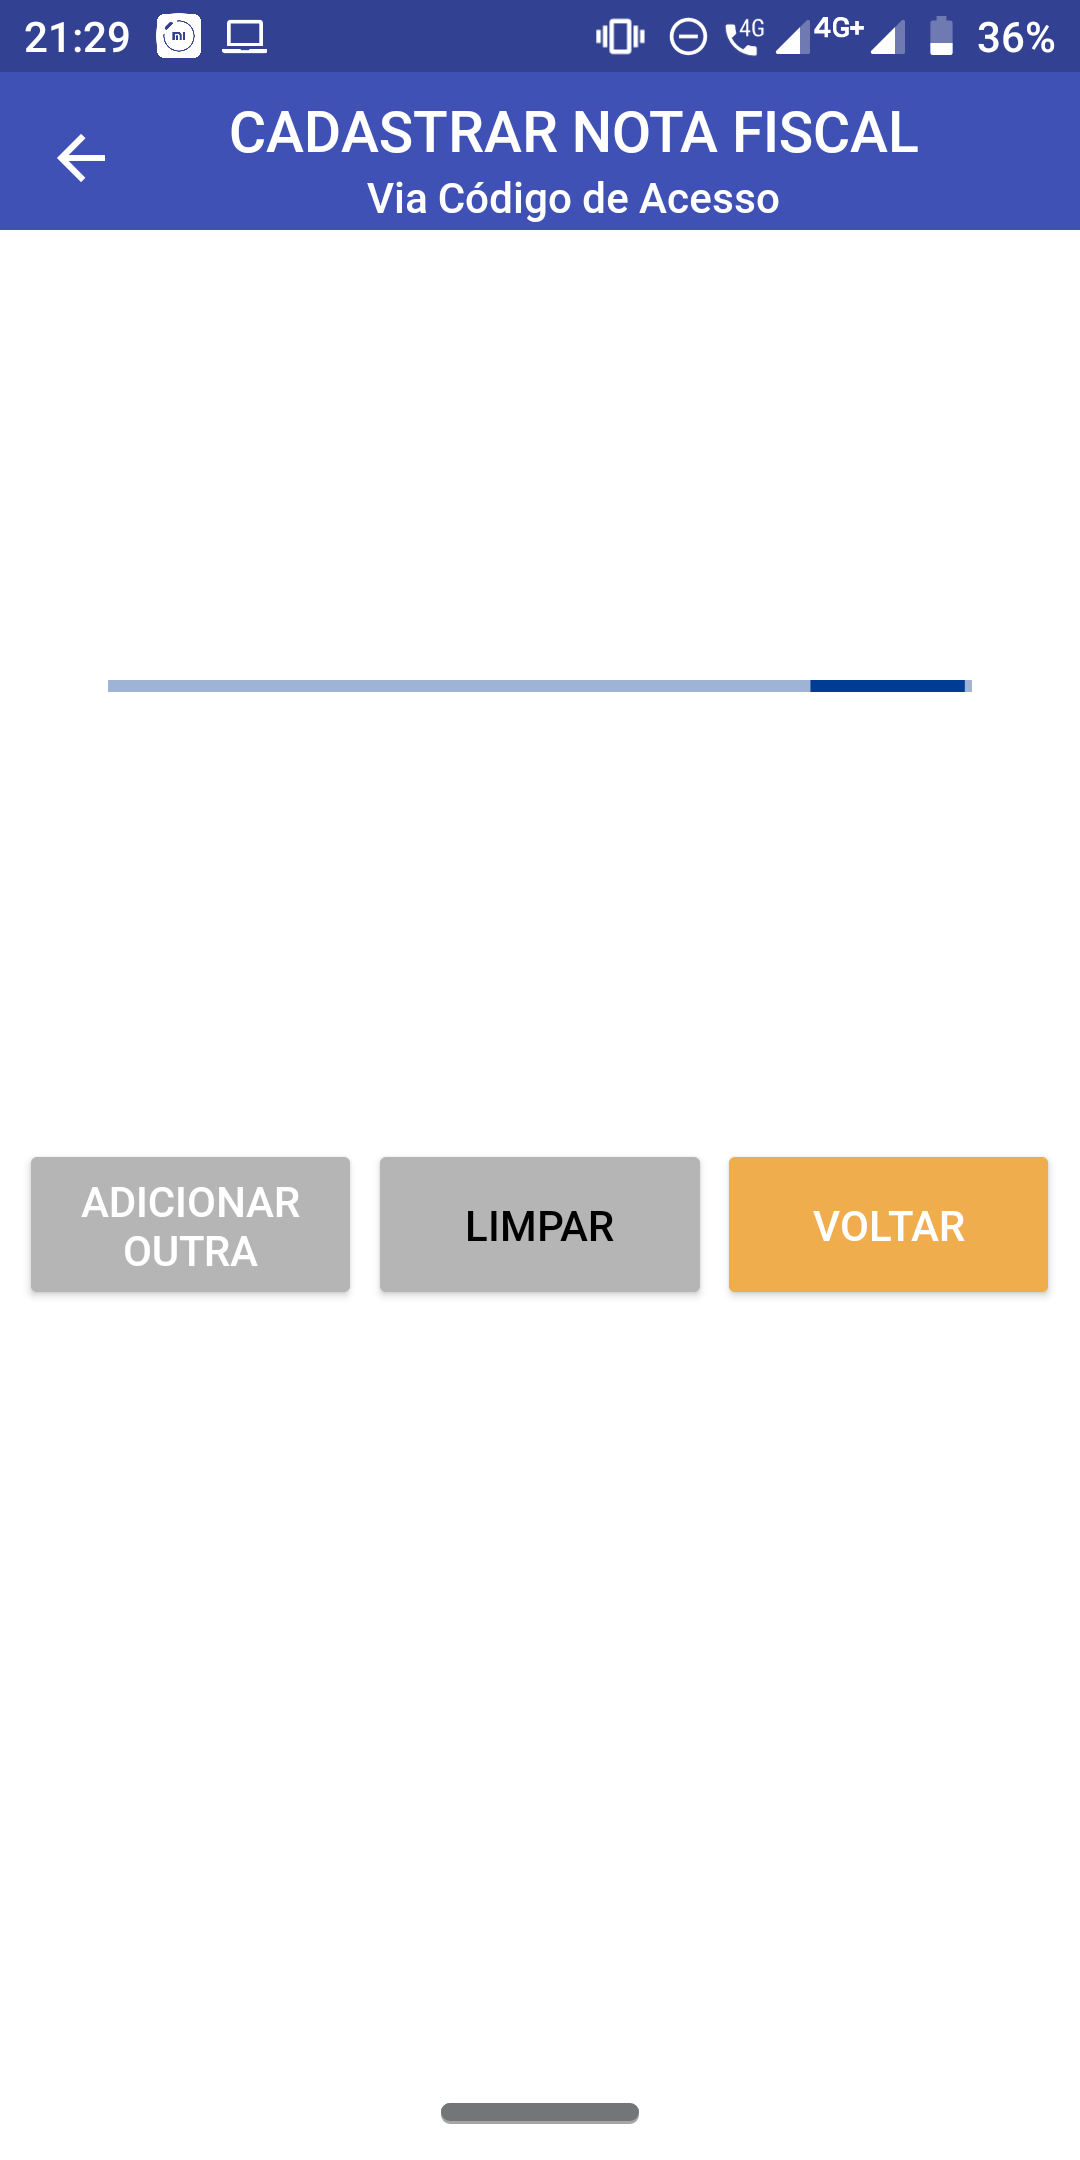
\includegraphics[scale=0.15]{tcc/figures/app/app_codigo_acesso_loading_solicitacao.png}
    \caption{Tela de cadastro via código de acesso após solicitação}
    \label{appCodigoAcessoLoadingSolicitacaoFig}
\end{figure}

Ao receber a resposta, o aplicativo irá mostrar diferentes telas dependendo do que resultado obtido. As telas são semelhantes ao serem comparadas com o outro método de adição de notas. No entanto, a principal diferença é que as telas para esse tipo de adição, os botões são diferentes. A primeira opção, também em azul, permite adicionar outra nota também por meio do código de acesso. O botão do meio, de limpar, é exibido de forma bloqueada pois não existem campos de inserção de dados nessa parte de resultados. Por fim, o último botão, em amarelo, permite que o usuário retorne para a tela inicial da aplicação.

\newpage
% FIXME: Ajustar a imagem
% FIXME: Adicionar referencia a imagem
\begin{figure}[h]
    \centering
    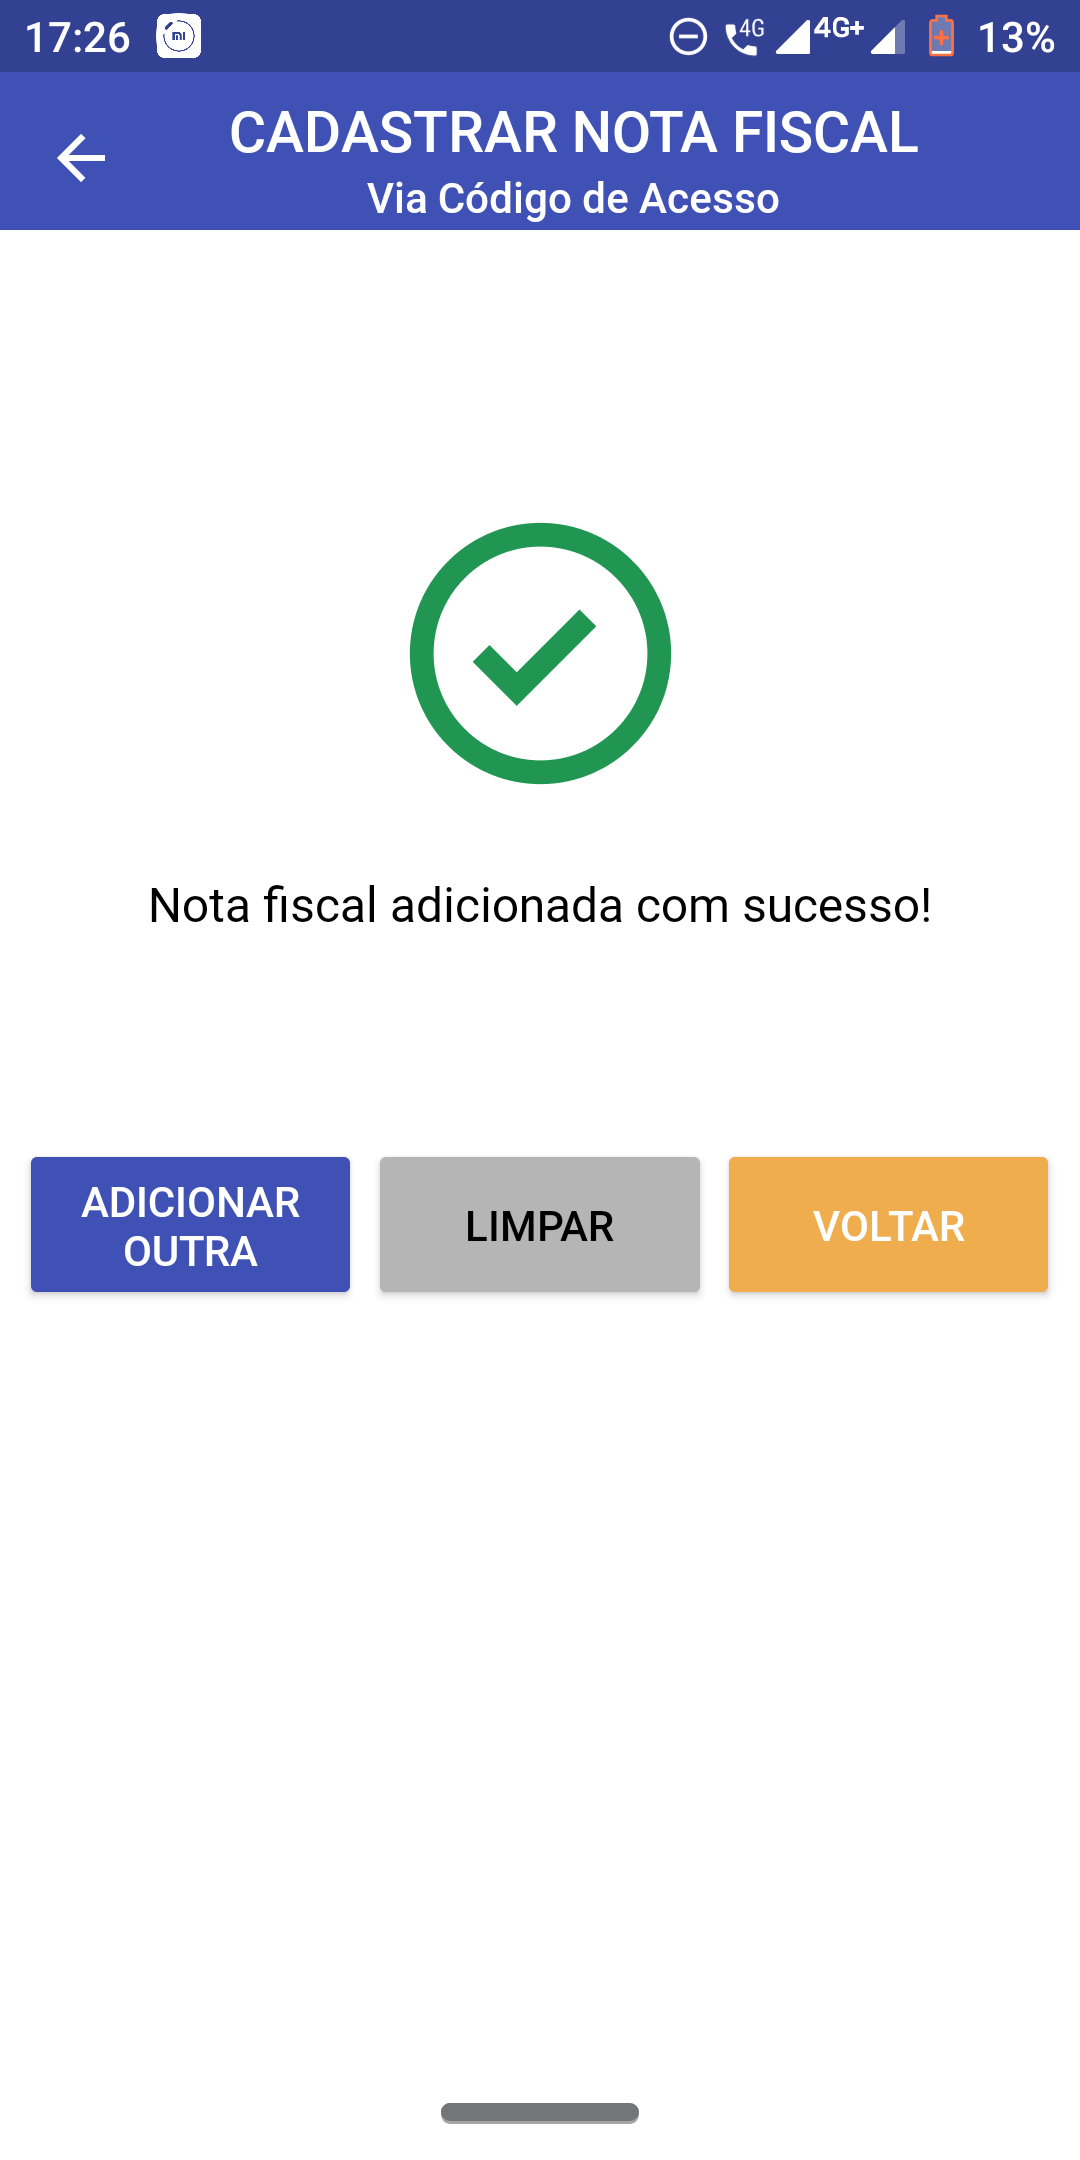
\includegraphics[scale=0.15]{tcc/figures/app/app_codigo_acesso_sucesso.png}
    \caption{Tela de cadastramento via código de acesso efetuado com sucesso}
    \label{appCodigoAcessoSucessoFig}
\end{figure}

\newpage
% FIXME: Ajustar a imagem
% FIXME: Adicionar referencia a imagem
\begin{figure}[h]
    \centering
    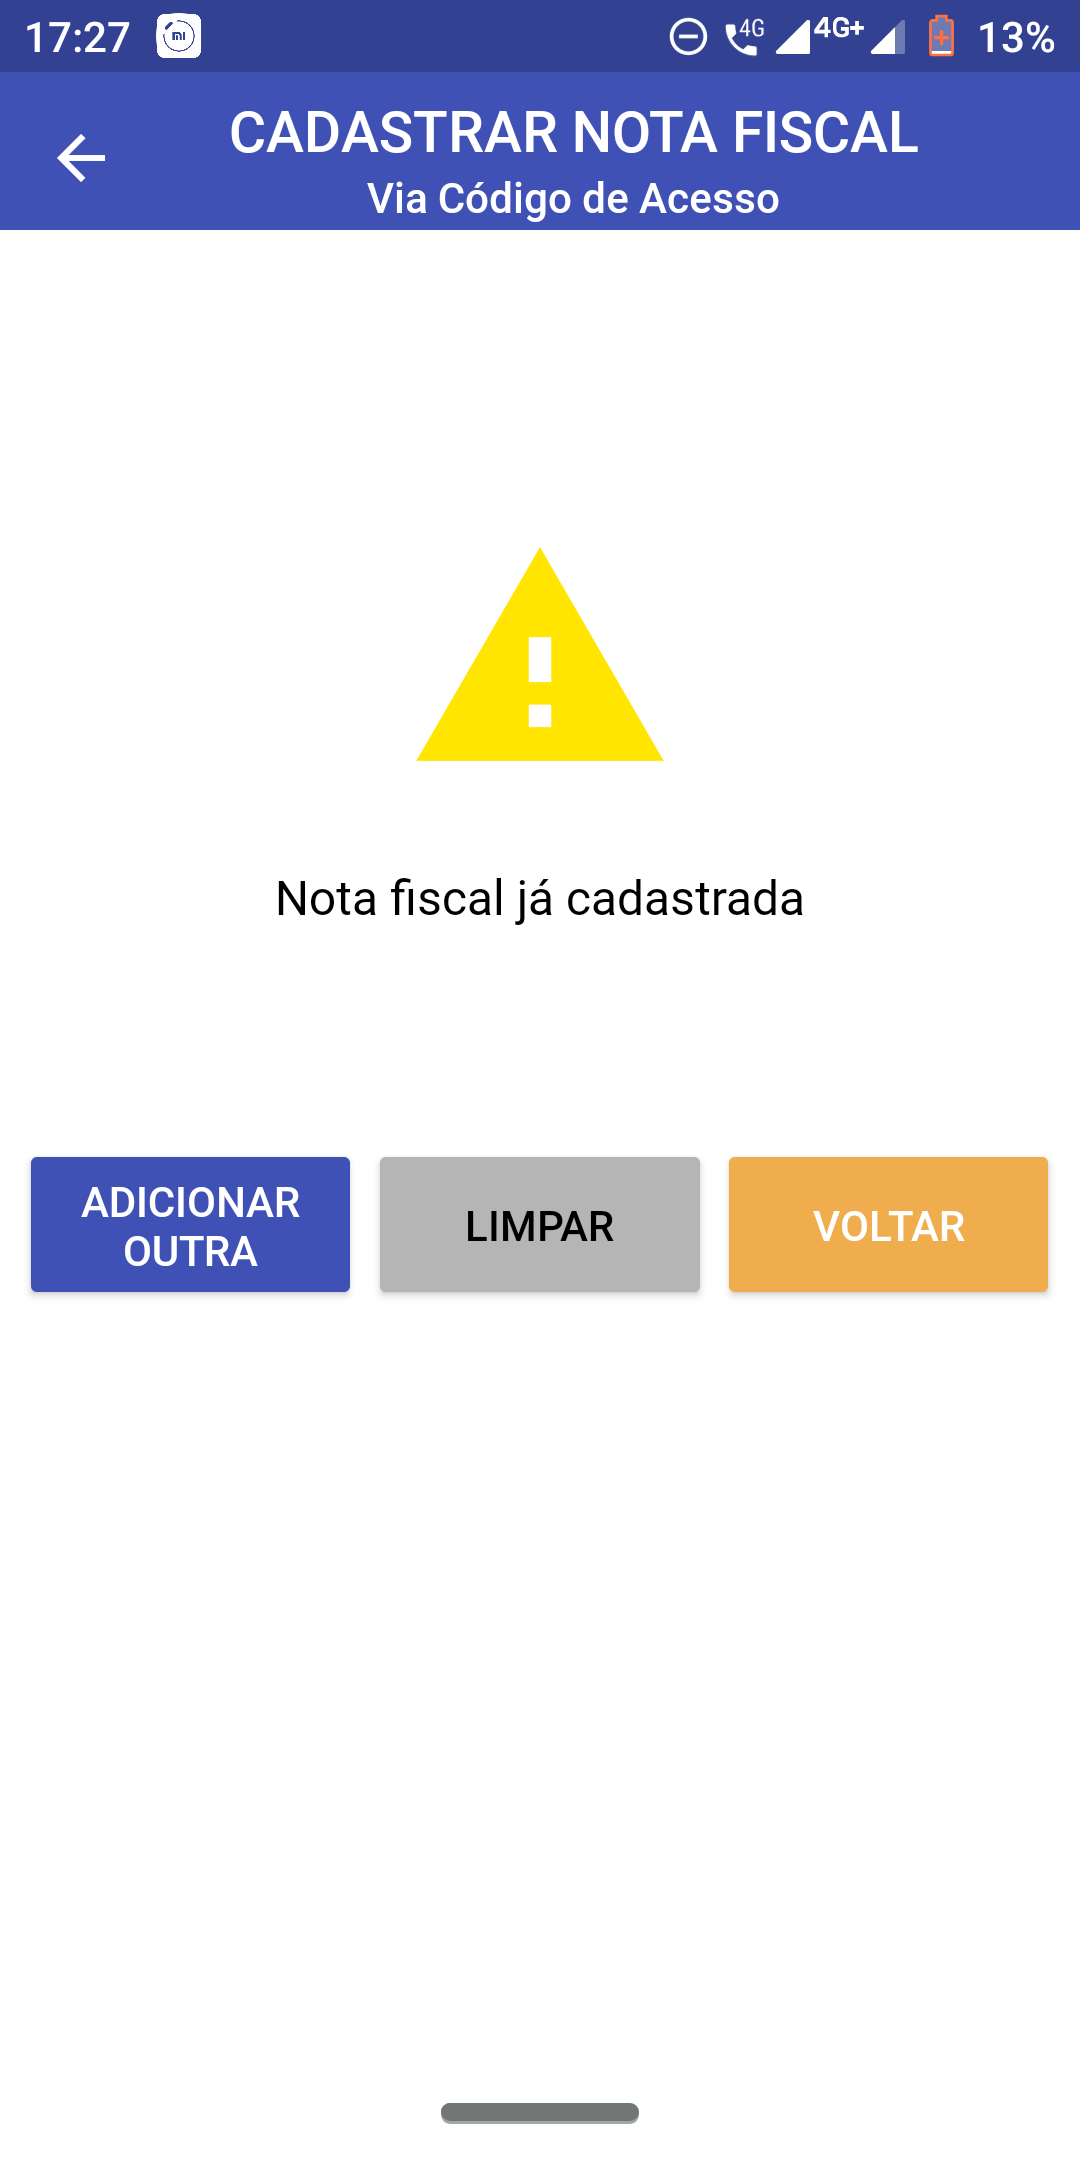
\includegraphics[scale=0.15]{tcc/figures/app/app_codigo_acesso_ja_cadastrada.png}
    \caption{Tela de cadastramento via código de acesso de uma nota cadastrada previamente}
    \label{appCodigoAcessoJaCadastradaFig}
\end{figure}

\newpage
% FIXME: Ajustar a imagem
% FIXME: Adicionar referencia a imagem
\begin{figure}[h]
    \centering
    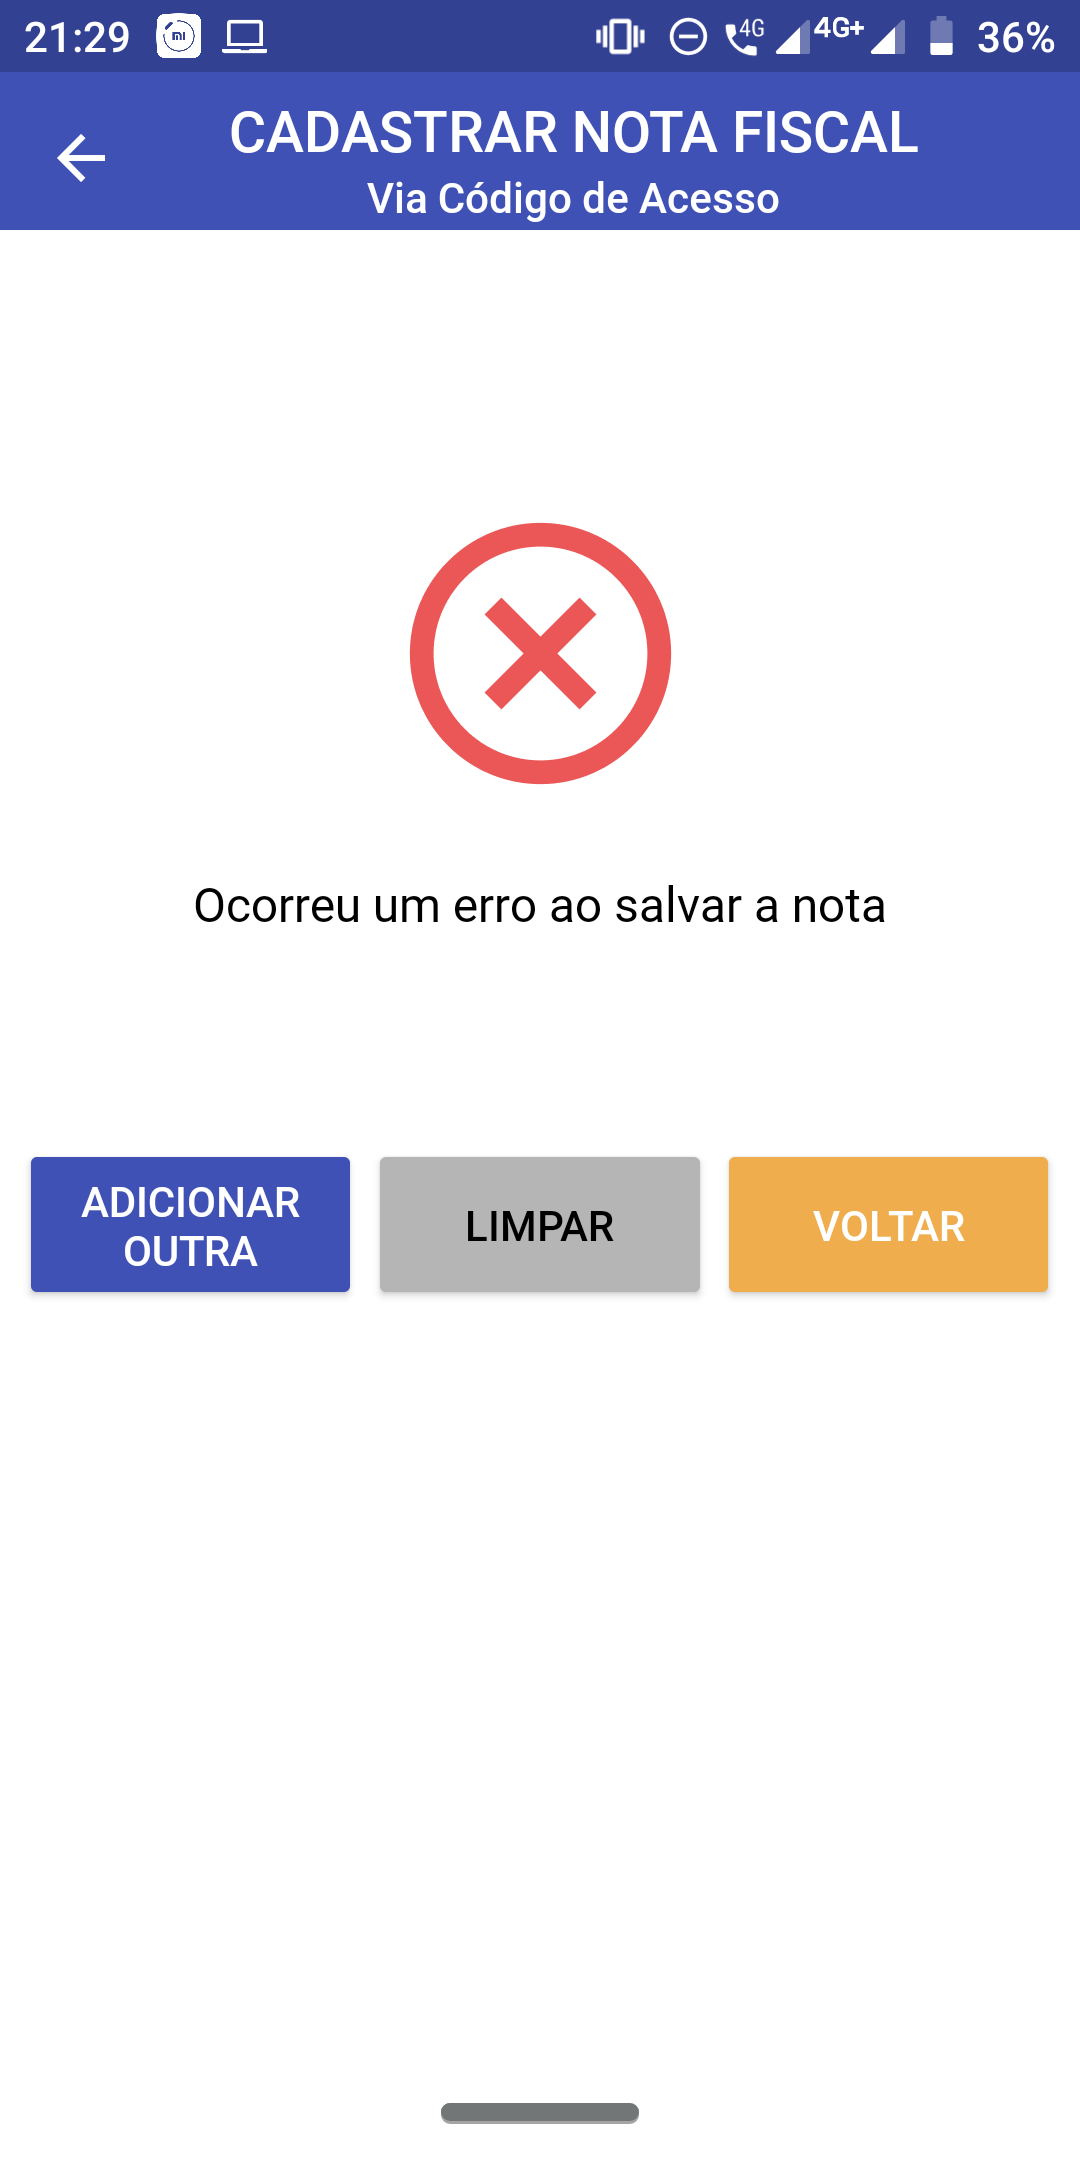
\includegraphics[scale=0.15]{tcc/figures/app/app_codigo_acesso_nao_disponivel.png}
    \caption{Tela de cadastramento via código de acesso de uma nota não disponível}
    \label{appCodigoAcessoNaoDisponivelFig}
\end{figure}

\newpage
% FIXME: Ajustar a imagem
% FIXME: Adicionar referencia a imagem
\begin{figure}[h]
    \centering
    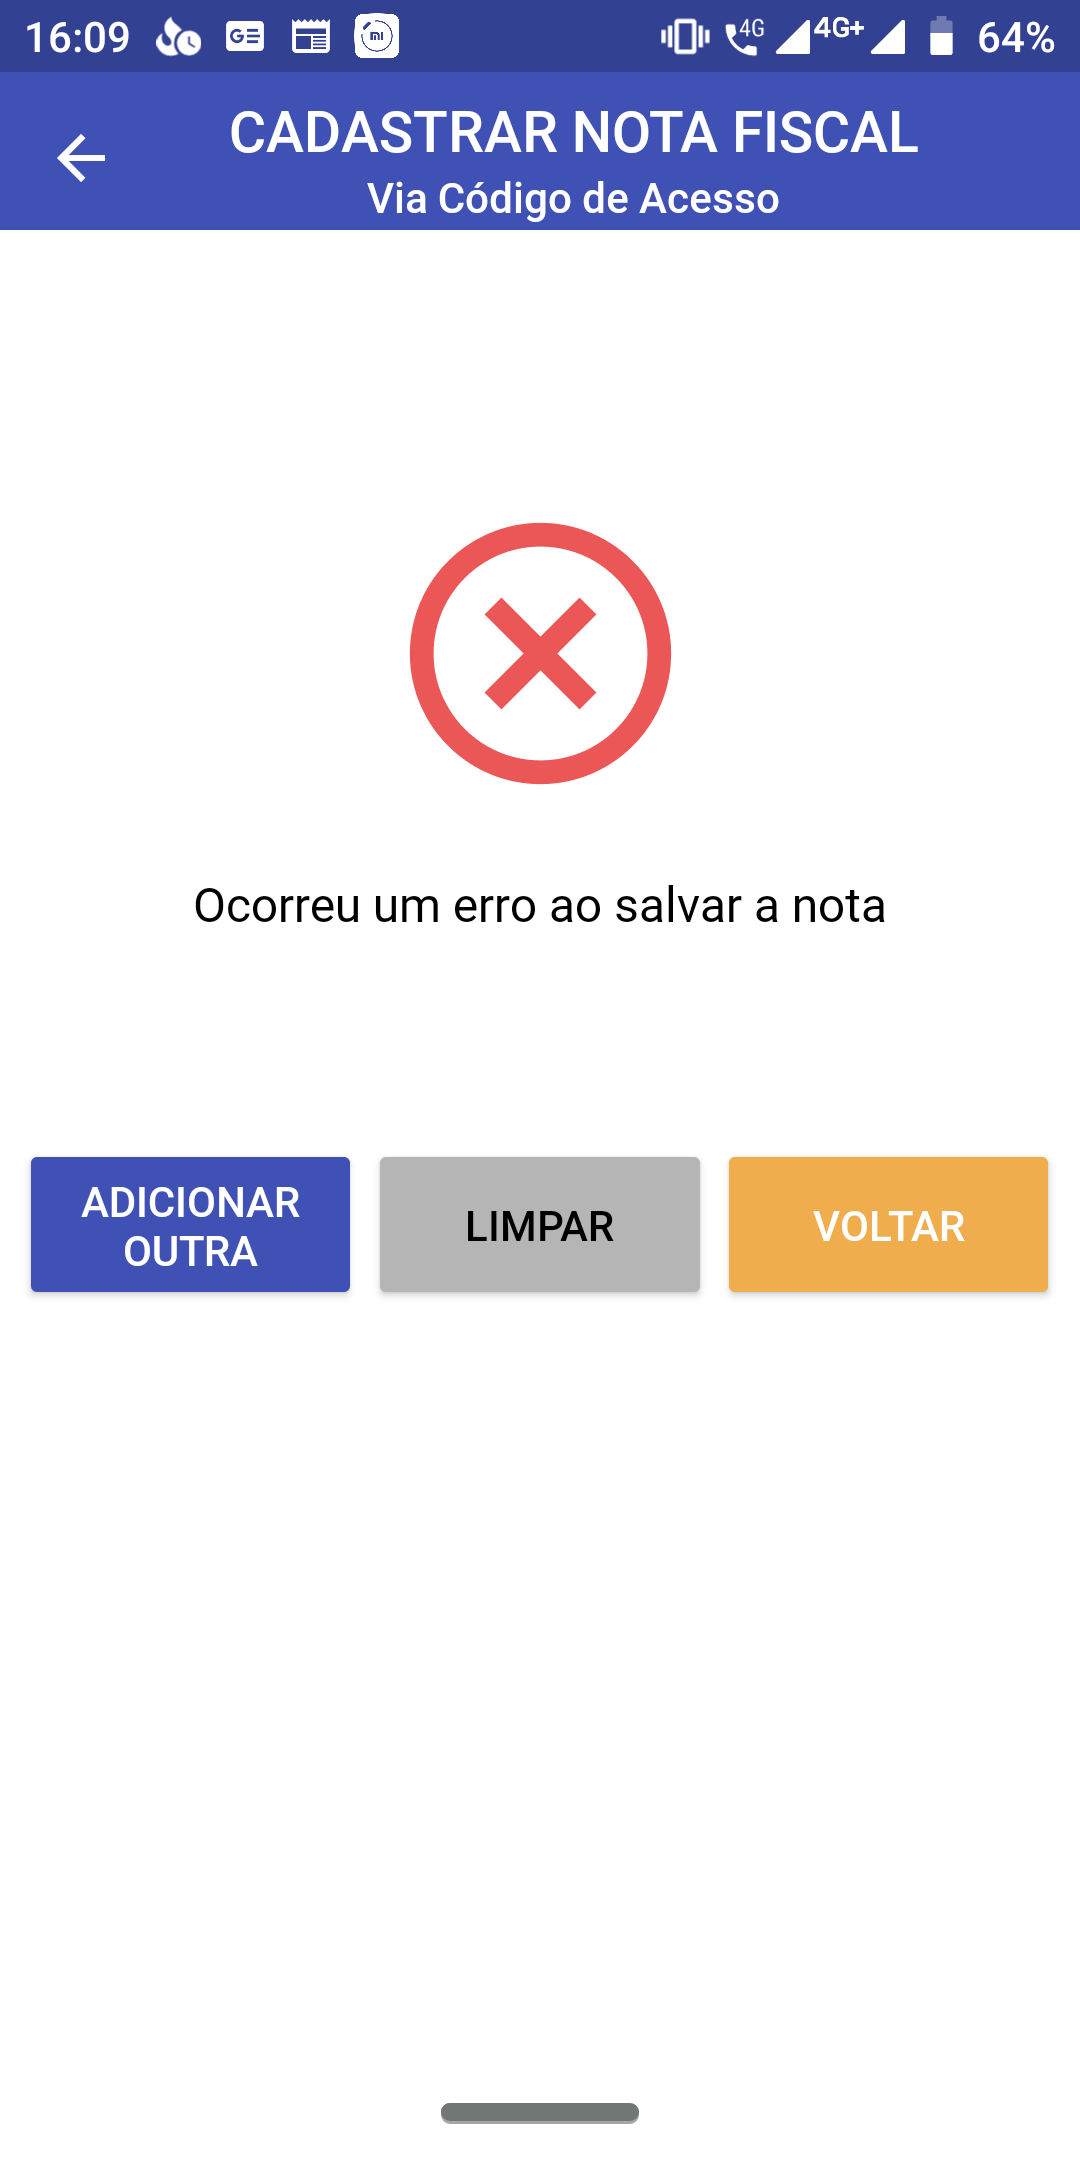
\includegraphics[scale=0.15]{tcc/figures/app/app_codigo_acesso_erro_generico.png}
    \caption{Tela de cadastramento via código de acesso após erro durante solicitação}
    \label{appCodigoAcessoErroFig}
\end{figure}

\newpage
% FIXME: Ajustar a imagem
% FIXME: Adicionar referencia a imagem
\begin{figure}[h]
    \centering
    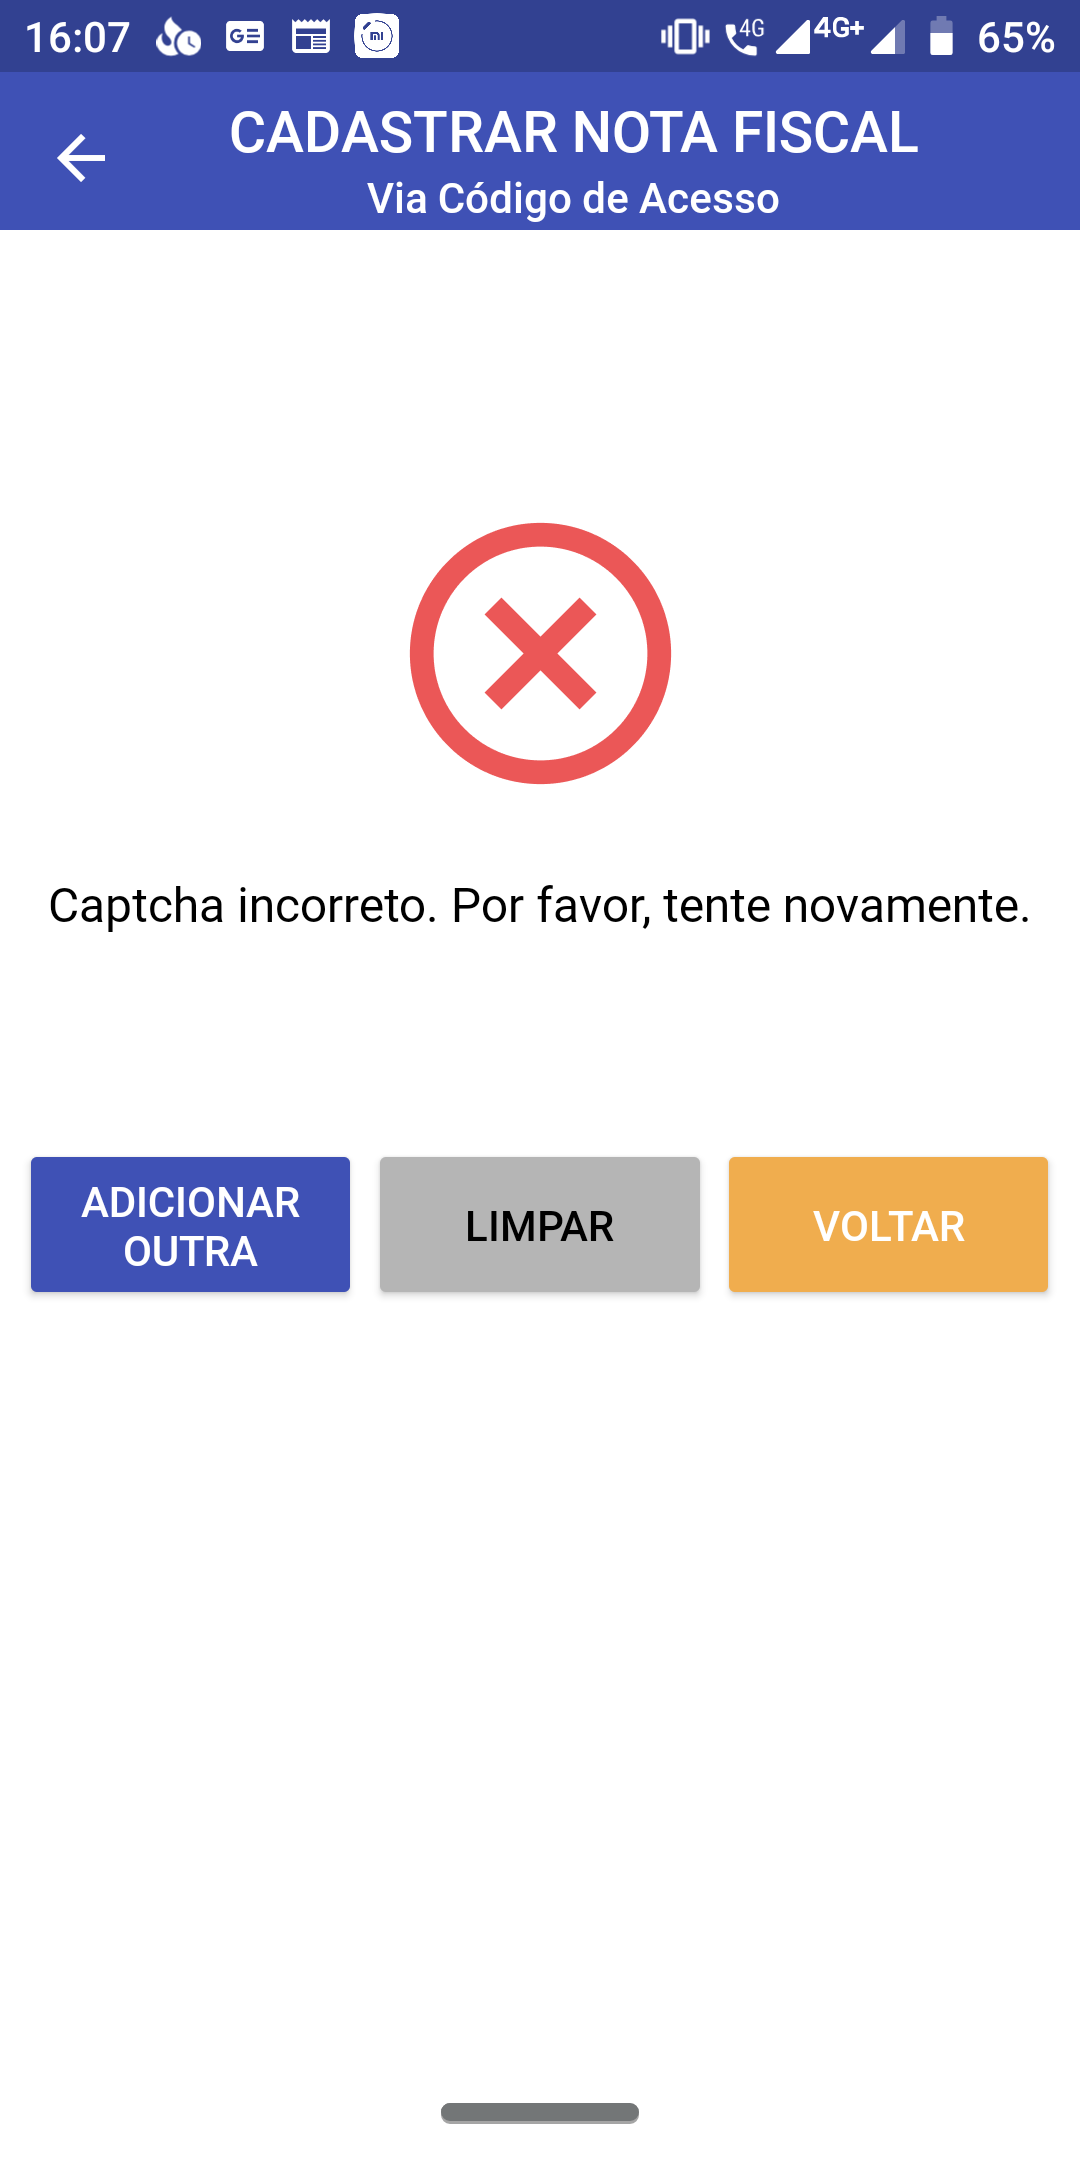
\includegraphics[scale=0.15]{tcc/figures/app/app_codigo_acesso_erro_captcha.png}
    \caption{Tela de cadastramento via código de acesso após inserção falha no teste do CAPTCHA}
    \label{appCodigoAcessoErroCaptchaFig}
\end{figure}

Existe uma tela diferente das demais quando comparado aos resultados do cadastro via QRCode. Isso ocorre devido a presença do campo para inserção do CAPTCHA, com isso deverá ter um tratamento para o erro do caso em que o usuário tenha inserido um texto diferente daquele presente na imagem. Esse erro resulta em uma falha no teste de validação, o que impede o término do processo de cadastro via esse meio.

\subsection{Busca de produtos}

Ao clicar no último botão da tela inicial, conforme visto na figura \ref{appHomeFig}, o usuário será encaminhado para a tela de busca de produtos. É através dessa tela que os usuários poderão consultar a informação referente aos produtos desejados cadastrados previamente. A tela em questão é apresentada pela figura \ref{appBuscaProdutosInicialFig}.

% FIXME: Ajustar a imagem
% FIXME: Adicionar referencia a imagem
\newpage
\begin{figure}[h]
    \centering
    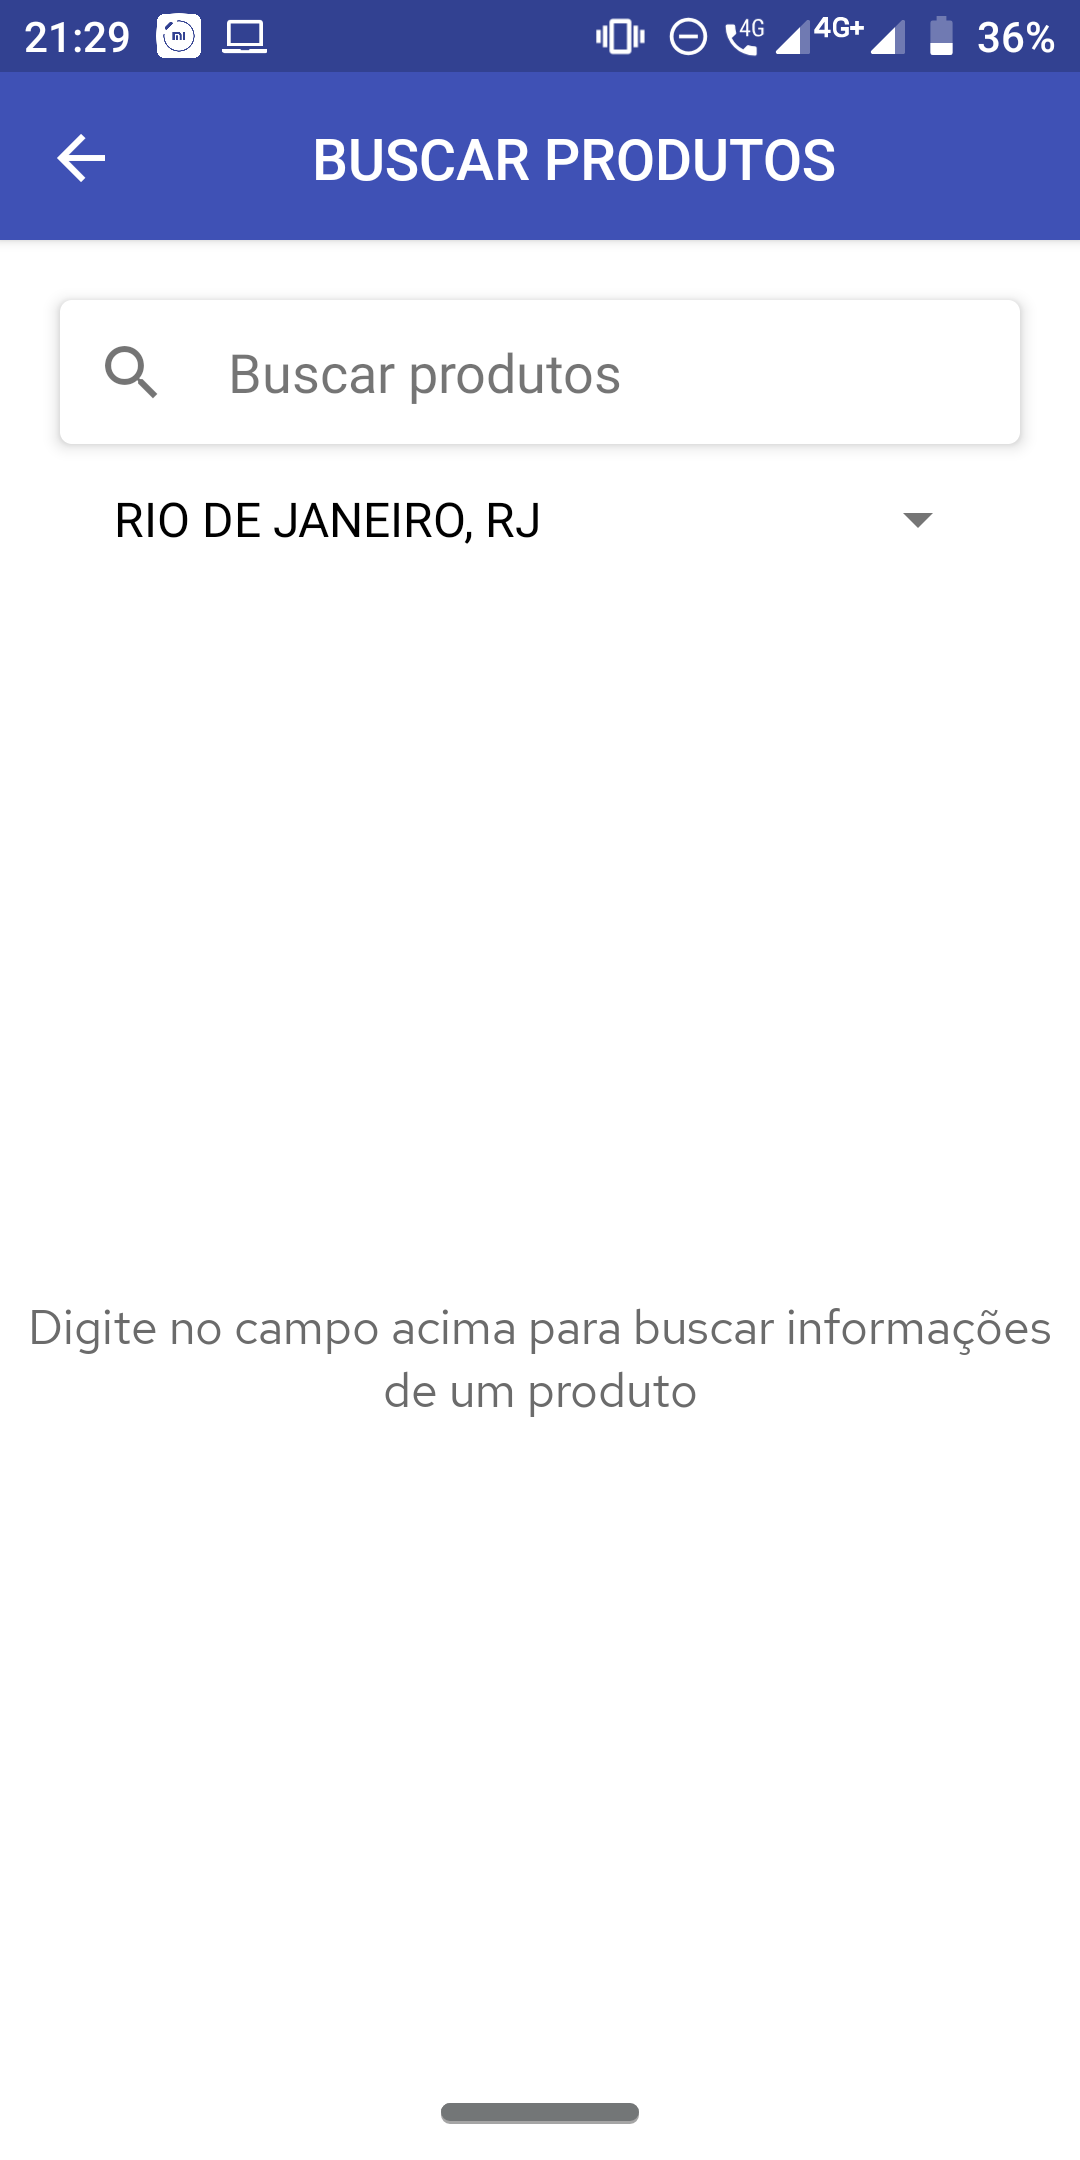
\includegraphics[scale=0.15]{tcc/figures/app/app_buscar_produtos.png}
    \caption{Tela para a realização da busca de produtos}
    \label{appBuscaProdutosInicialFig}
\end{figure}

Logo no início da tela, consta o campo que será utilizado para a inserção do texto referente aos nomes dos produtos. Ao lado esquerdo do campo, existe um ícone no formato de uma lupa que permitirá que o usuário toque para a realização da busca.

Abaixo do campo de texto, existe uma caixa de seleção para que o usuário consulte as cidades disponíveis para busca. Os nomes das cidades são recuperados a partir das notas que foram cadastradas previamente. Além disso, é permitido ao usuário escolher a opção de efetuar a busca em todas as cidades. A figura \ref{appBuscaProdutosCidadesFig} demonstra um exemplo de cidades disponíveis na caixa de seleção para a busca dos produtos.

No meio da tela, constará informações para auxílio ao usuário dependendo da situação em que a tela se encontra. Como pode ser observado na figura \ref{appBuscaProdutosInicialFig}, consta uma breve instrução de como o usuário deve efetuar sua busca. Ademais, caso o produto buscado não seja encontrado na base de dados, nessa mesma área será mostrada a mensagem que os produtos não foram localizados.

% FIXME: Ajustar a imagem
% FIXME: Adicionar referencia a imagem
\begin{figure}[h]
    \centering
    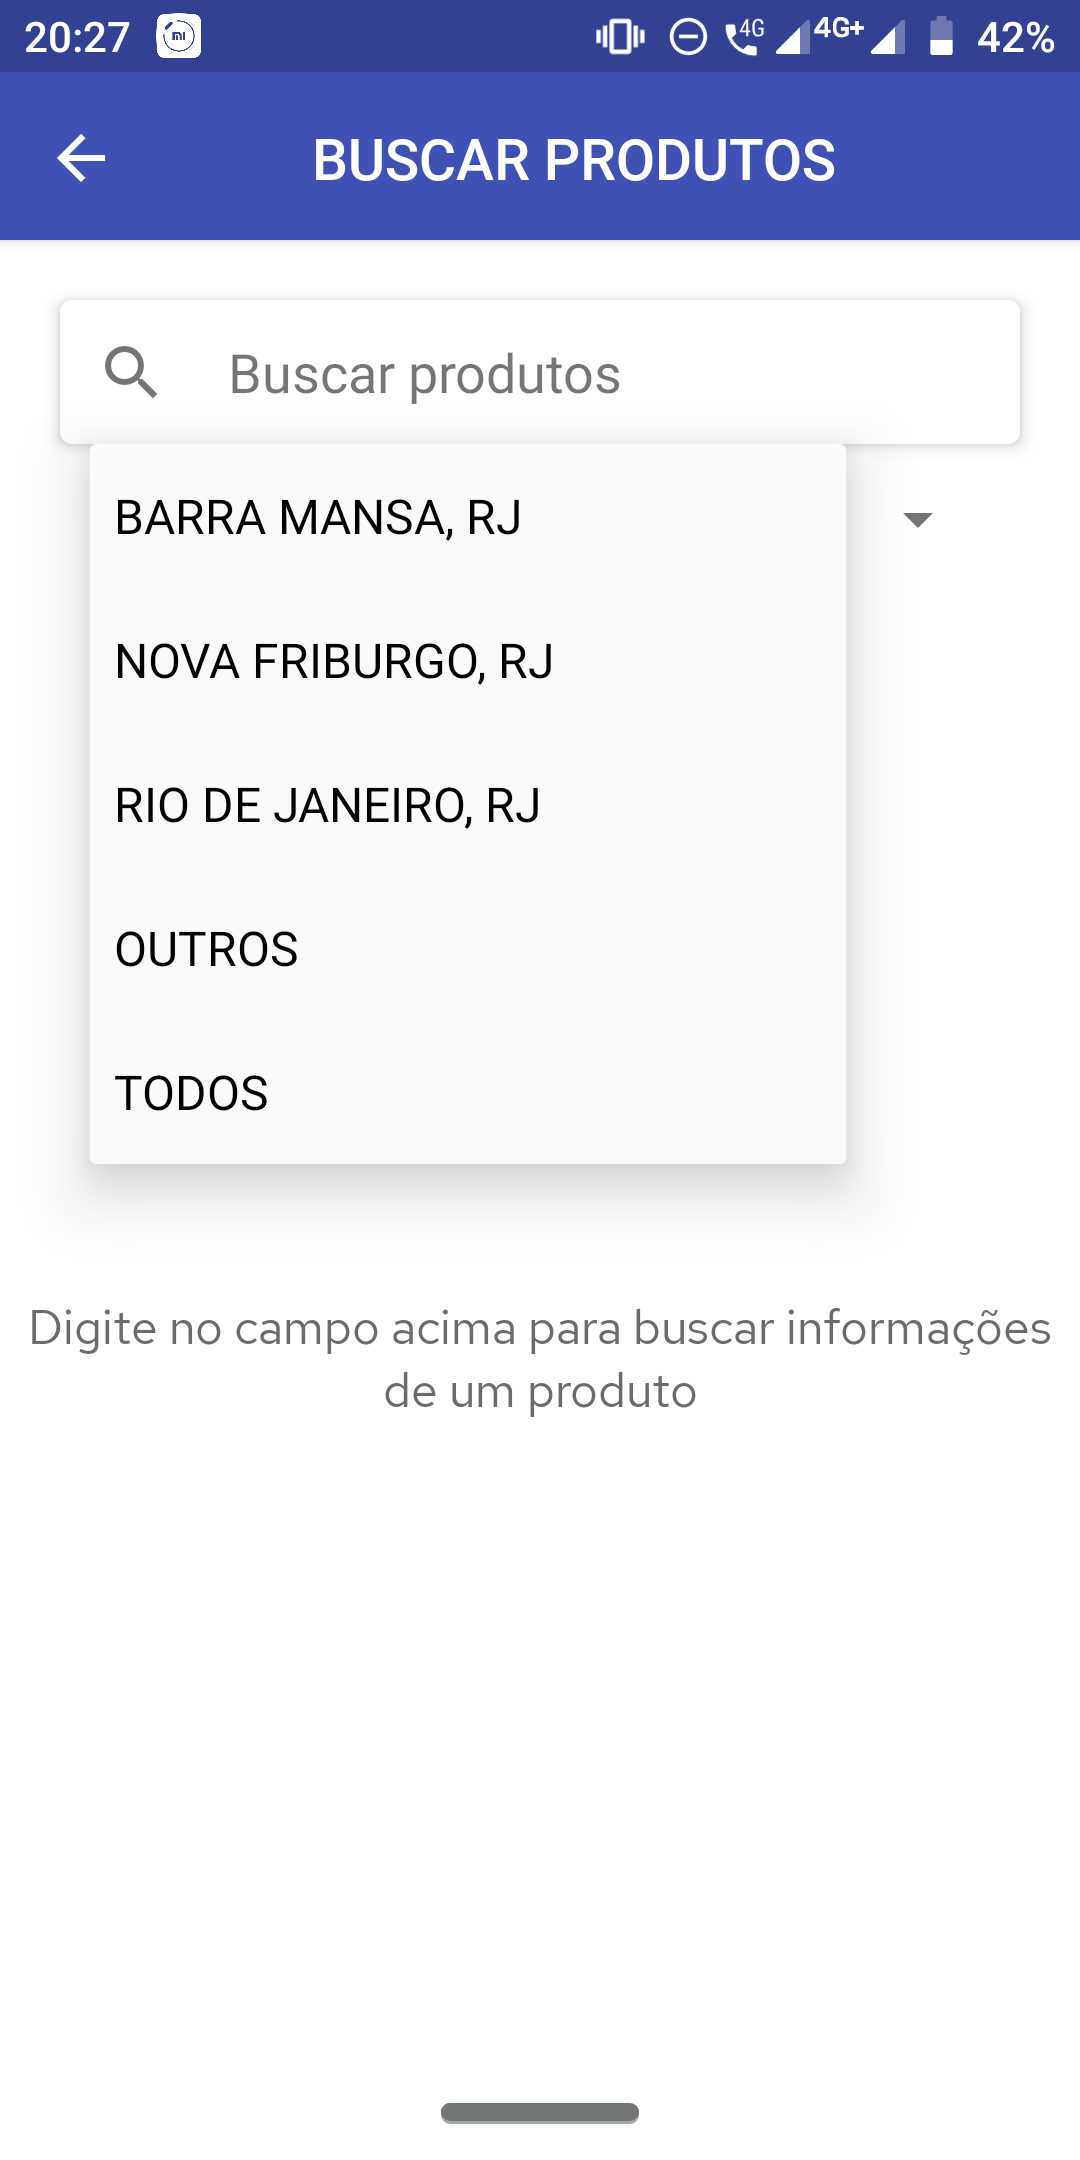
\includegraphics[scale=0.15]{tcc/figures/app/app_buscar_produtos_cidades.png}
    \caption{Exemplo de cidades disponíveis para busca de produtos}
    \label{appBuscaProdutosCidadesFig}
\end{figure}

\newpage
Após a escolha da cidade em que será efetuada a busca, o usuário deverá inserir o nome do produto que deseja buscar no campo de texto dedicado. Vale destacar que o usuário poderá inserir o texto escrito corretamente ou totalmente sem acentuação, e até mesmo com todas as letras em maiúsculo que será retornado o mesmo resultado do cenário em que o usuário escreveu corretamente.

\newpage
% FIXME: Ajustar a imagem
% FIXME: Adicionar referencia a imagem
\begin{figure}[h]
    \centering
    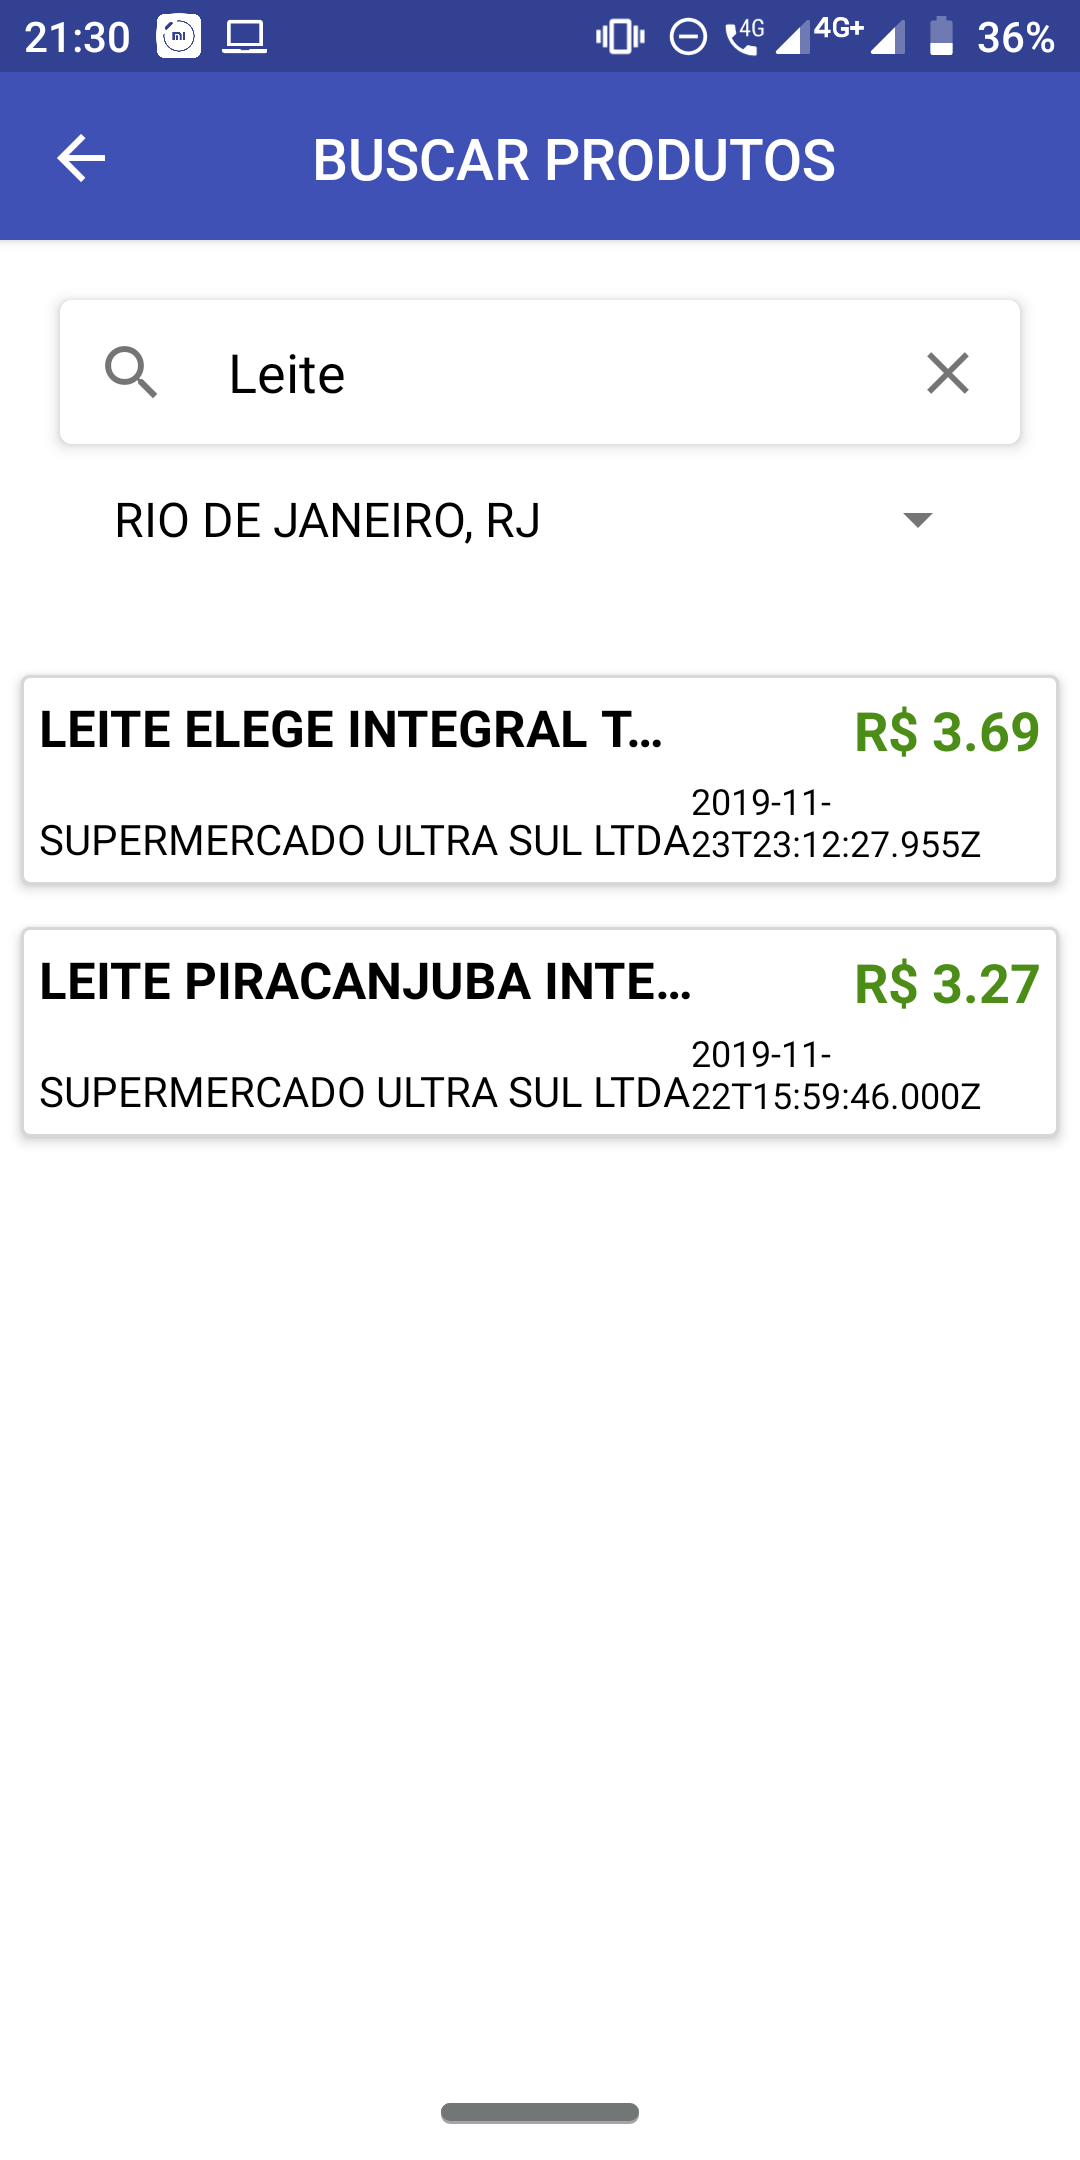
\includegraphics[scale=0.15]{tcc/figures/app/app_buscar_produtos_busca.png}
    \caption{Resultado de uma busca de um produto}
    \label{appBuscaProdutosBuscaResultadoFig}
\end{figure}

Um exemplo de uma busca pelo produto "Leite" é mostrada na figura \ref{appBuscaProdutosBuscaResultadoFig}. Como pode ser observado foram retornados dois registros para esse mesmo produto. Nessa busca, foram encontrados o mesmo produto no entanto de marcas diferentes, além disso, é possível efetuar uma comparação de preços, como também em que dia foi efetuada a compra dos mesmos.

Vale destacar que ambos os produtos foram comprados no mesmo supermercado, no entanto, o nome aparece cortado devido a uma limitação da largura do dispositivo utilizado para efetuar a captura da tela. No entanto, como o nome do mercado pode ser uma cadeia longa de caracteres, esse problema pode ser contornado pois é fornecida uma opção do usuário visualizar as informações completas referentes ao registros individuais dos produtos, para isso, basta efetuar um toque no campo referente ao produto que uma pop-up surgirá em tela contendo as mesmas informações fornecidas anteriormente, no entanto, 
como é possível ocupar a maior parte do espaço disponível em tela, será possível visualizar todas as informações que foram ocultadas anteriormente. Além do nome do local da compra, o próprio nome do produto poderá ser cortado caso esse também seja extenso. Por fim, um exemplo dessa solução descrita anteriormente pode ser observada na figura \ref{appBuscaProdutosProdutoAmpliadoFig}.

% FIXME: Ajustar a imagem
% FIXME: Adicionar referencia a imagem
\begin{figure}[h]
    \centering
    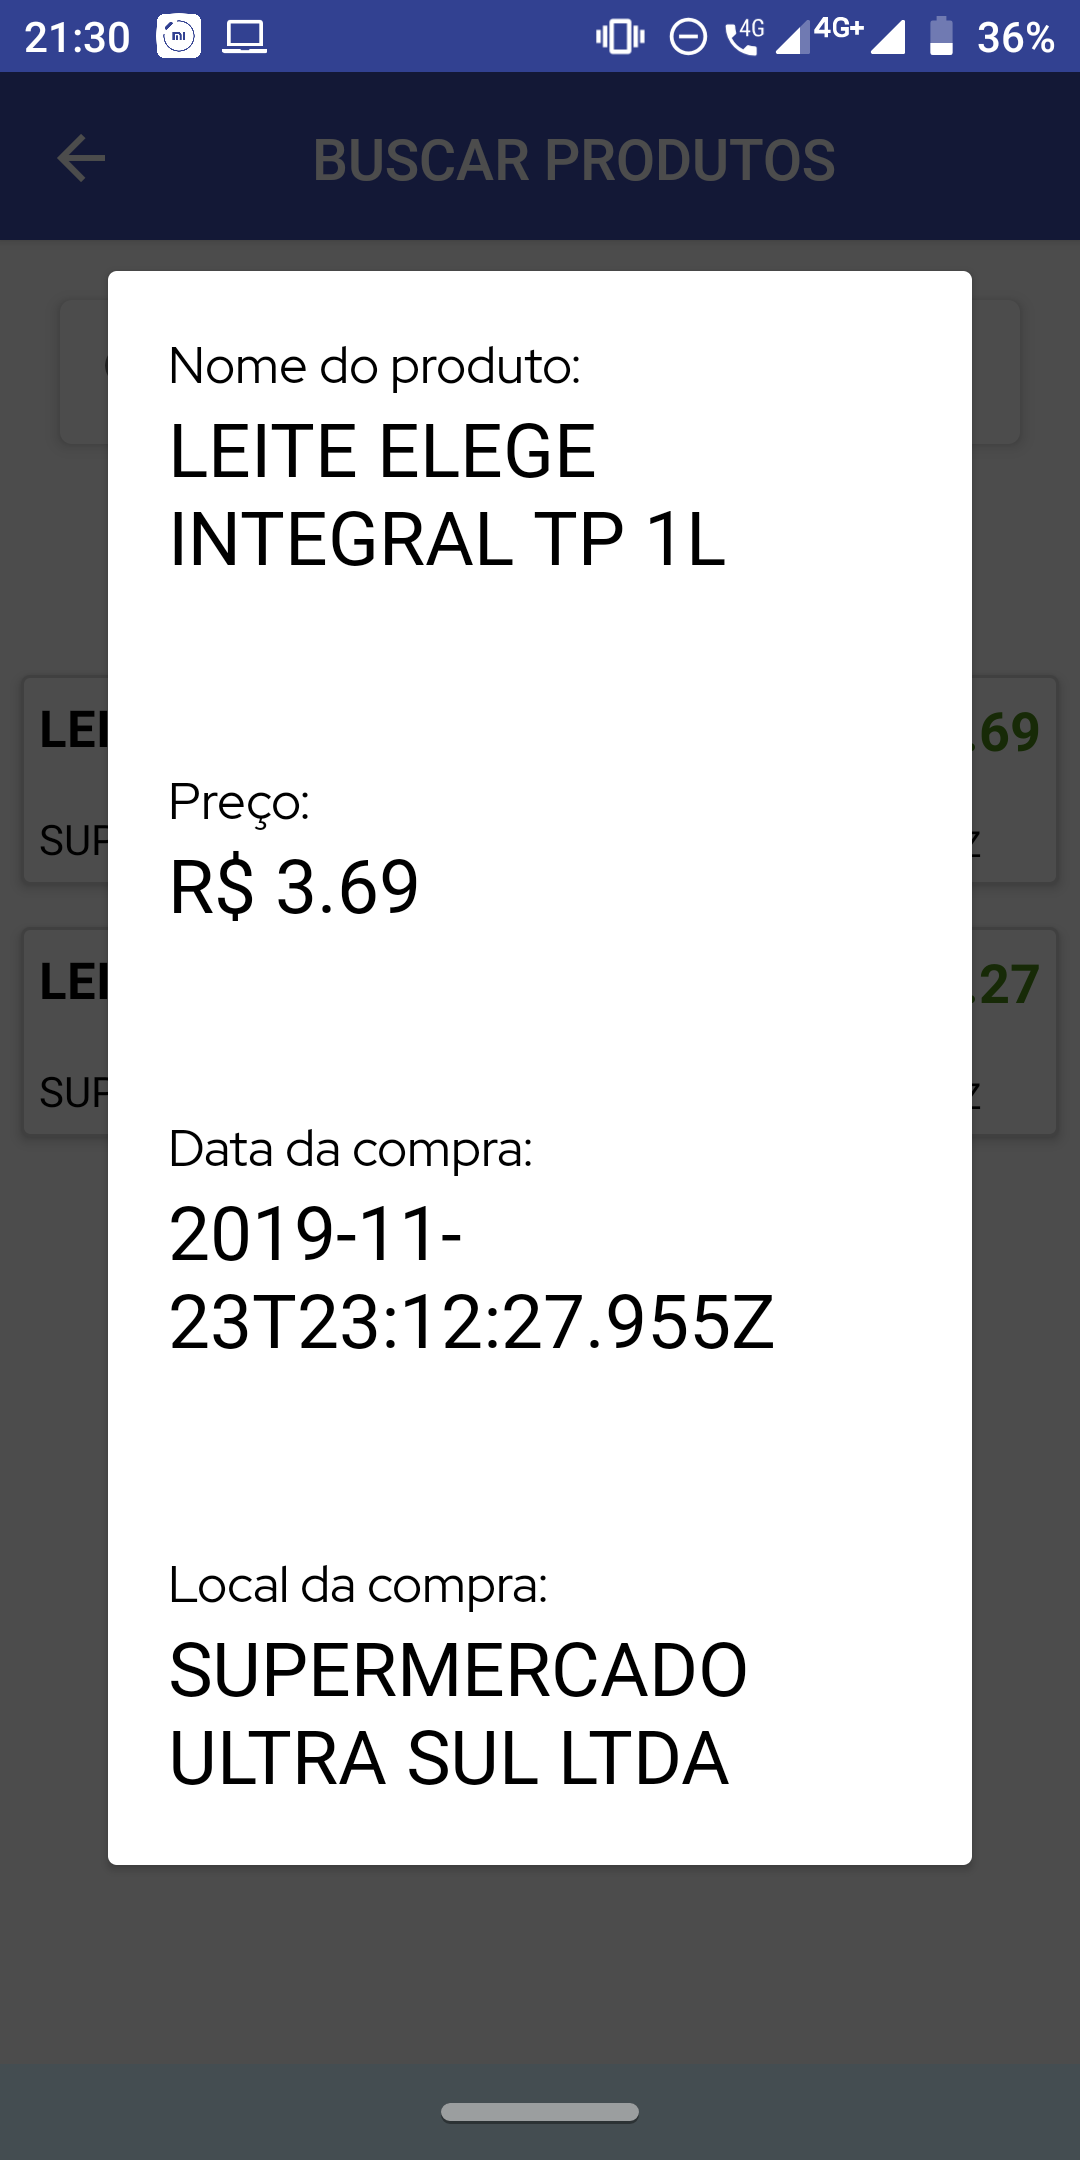
\includegraphics[scale=0.15]{tcc/figures/app/app_buscar_produtos_produto.png}
    \caption{Exemplo de um produto com suas informações disponibilizadas em uma pop-up.}
    \label{appBuscaProdutosProdutoAmpliadoFig}
\end{figure}

\section{Prós e contras do desenvolvimento}

Uma vantagem durante o desenvolvimento, foi que tanto o aplicativo quanto o código do servidor, isto é, a API, foram desenvolvidos utilizando a mesma linguagem de programação, logo, houve uma melhor integração entre as partes.

Alguns problemas ocorreram durante o desenvolvimento da aplicação e da API, como exemplo, pode ser citado que ao efetuar a busca por produtos, todos os produtos contidos na nota fiscal eram retornados. Além disso, durante a busca, a partir do produto não estava sendo possível retornar o local onde o mesmo foi comprado e também, não estava sendo retornando o último registro por mercado, pois estava sempre retornando os registros em que tiveram os menores preços registrados.

Ainda ocorreram problemas durante o desenvolvimento das interfaces da aplicação, pois alguns botões estavam apresentando problemas nas funções que deveriam desempenhar como também o posicionamento dos elementos em tela.

\section{Limitações do aplicativo e das tecnologias utilizadas}

Assim como já foi dito em outros trechos desse trabalho, uma limitação existente na versão atual do aplicativo é que não é possível efetuar a instalação do mesmo a partir das lojas oficias das plataformas suportadas, isto é, a Play Store e a App Store.

Além disso, só é suportado o cadastro de notas fiscais emitidas no Estado do Rio de Janeiro. Ainda relacionado com as notas, o aplicativo apresenta dificuldades de leitura de QRCodes que tiveram problemas durante a impressão.

Por fim, vale observar que o cadastro de notas e a recuperação das informações somente podem ser feitas caso o dispositivo que estiver executando a aplicação esteja conectado à internet.

\subsection{Desvantagem do tipo de banco de dados utilizado}

Uma desvantagem do tipo de banco de dados não-relacional, o qual foi utilizado nesse projeto, é que não foi possui a mesma consistência presente em bancos do tipo relacional, porém, como a informação mais relevante durante a busca dos dados é sempre o último registro efetuado para um produto, logo isso não se torna um problema para o projeto, pois o último registro é sempre garantido.

\section{Obtenção do aplicativo e atualizações}

O autor desse trabalho possui a intenção de efetuar a publicação do aplicativo nas lojas oficias das plataformas suportadas pela aplicação. Conforme, discutido na \autoref{sec-app-desenvolvido}, é possível instalar uma versão funcional do aplicativo, semelhante a que será publicada, em dispositivos que rodam o sistema Android. Vale ressaltar que a prática de instalar aplicativos fora das lojas oficias não é recomendada devido a brechas de segurança. Com isso, o autor se compromete em fornecer um aplicativo seguro que não causará danos ao sistema operacional dos usuários nessa versão prévia do projeto.

Sobre as atualizações com melhorias e correções, poderão ser obtidas de duas formas diferentes, primeiramente dar-se-a através das próprias lojas de aplicativos, após a publicação nas mesmas, já a segunda forma é através do uso de atualizações \textit{Over-the-air} (OTA, em tradução livre: "Por via aérea"), que é um tipo de atualização que o próprio aplicativo efetua o download e realiza a instalação da mesma. Esse recurso é fornecido pela ferramenta Expo e permite que o usuário possua a versão mais atualizada do aplicativo sempre que possível. Por padrão, é efetuada uma verificação por novas atualizações a cada 30 dias. Por fim, por meio dessa última forma é possível ter acesso a versões mais atualizadas do aplicativo sem ser através dos lojas das plataformas.

\section{Trabalhos futuros}

Embora o aplicativo tenha atingido o objetivo principal, que era o cadastro das notas fiscais e a recuperação dos preços dos produtos contidos nas mesmas, novas funcionalidades podem ser incluídas de forma a melhorar ainda mais a experiência do usuário e facilitar mais ainda o cotidiano dos cidadãos. Como por exemplo, pode ser adicionado o suporte ao sistema de outros estados fazendo com que mais brasileiros possam utilizar o aplicativo não ficando limitado somente à população do Estado do Rio de Janeiro.

Além disso, melhorias poderão ser realizadas durante o processo de leitura do QRCode, isto é, uma vez que possa ser impresso em uma qualidade ruim poderá ocasionar problemas durante a leitura, fazendo com que a mesma não seja realizada com sucesso. De forma a contornar esse problema, poderá ser efetuado um pós-processamento da imagem após um tempo gasto estipulado anteriormente, com isso, ainda será possível efetuar a adição da nota sem a necessidade de digitação de textos.

Ainda durante o processo de leitura do QRCode, se após o processamento da imagem não for possível concluir a leitura e a obtenção da informação, poderá ser oferecido ao usuário a opção de adição através do código de acesso automaticamente caso o aplicativo detecte que há uma demora para efetuar a leitura.

Por fim, uma outra melhoria que poderá ser implementada, é uma outra forma de notificação ao usuário que sua nota foi processada fazendo com que o mesmo possa utilizar outros aplicativos não sendo mais necessário permanecer com uma das telas de cadastro abertas aguardando a resposta. Com isso, poderá ser adicionada mais de uma nota por vez, o que melhorá ainda mais a serventia do projeto.